\documentclass[authoryear, review, 11pt]{elsarticle}

\setlength{\textwidth}{6.5in}
%\setlength{\textheight}{9in}
\setlength{\topmargin}{0in}
\setlength{\oddsidemargin}{0in}
\setlength{\evensidemargin}{0in}

\usepackage{amsmath}
\usepackage{amsthm}
\usepackage{amssymb}
\usepackage{mathabx}
\usepackage{bm}
\usepackage{multirow}

%\geometry{landscape}                % Activate for for rotated page geometry
\usepackage[parfill]{parskip}    % Activate to begin paragraphs with an empty line rather than an indent
\usepackage{graphicx}
\usepackage{epstopdf}
\usepackage{natbib}
\usepackage{verbatim}
\usepackage{longtable}
\usepackage[nolists,nomarkers]{endfloat}
\DeclareDelayedFloatFlavour*{longtable}{table}

\usepackage{relsize}
%\usepackage{caption}
\usepackage{subcaption}
\usepackage{fullpage}
\usepackage{booktabs}
\usepackage{rotating}

\usepackage{setspace}
\setstretch{2}

\DeclareGraphicsRule{.tif}{png}{.png}{`convert #1 `dirname #1`/`basename #1 .tif`.png}
\DeclareMathOperator*{\argmin}{\arg\!\min}
\DeclareMathOperator*{\argmax}{\arg\!\max}
\DeclareMathOperator*{\bw}{\mbox{bw}}
\DeclareMathOperator*{\df}{\mbox{df}}
\newcommand{\vect}[1]{\bm{#1}}
\newcommand{\E}{\mathop{\mathbb E}}


\title{Local Variable Selection and Parameter Estimation of Spatially Varying Coefficient Models for Geographically Weighted Regression}
\author{Wesley Brooks}
\date{}                                           % Activate to display a given date or no date

\begin{document}
\maketitle
%\section{}
%\subsection{}




%\begin{spacing}{2}
\section{Introduction}
	%Varying coefficient regression
	Varying coefficient regression (VCR) is a technique used to model non-stationary regression processes \citep{Hastie:1993a}. Whereas the coefficients in traditional linear regression are scalar constants, the coefficients in a VCR model are functions - often \emph{smooth} functions - of some effect modifying variable. When the effect modifying variable $\bm{s}$ represents location in a spatial domain, a VCR model implies that there is a local regression model $y(\bm{s}) = \bm{x}(\bm{s})' \bm{\beta}(\bm{s}) + \varepsilon(\bm{s})$ at each location $\bm{s}$. These local models are in contrast to a global linear regression model, where the coefficients are constant across the domain. Estimating the coefficient functions of a VCR model is therefore more complicated than estimating the coefficients in a global linear regression model.
	
	%Spatial data / spatial regression
	This document investigates an application of VCR models for spatial data where the effect-modifying variable is spatial location. It is a method for analyzing geostatistical data, which consists of observations of a continuous process, made at a set of discrete locations. The data example in section \ref{section:data-analysis} uses areal data, such as the poverty rate in a county, but treats it as geostatistical data by assuming that each measurement was made at the county's centroid.
	
	Spatial association - meaning that nearby locations are more alike than distant locations - is a key concept in spatial statistics. Common practice in the analysis of geostatistical data is to write a spatial model as the sum of systematic and random components, as in: 
\begin{align}\label{eq:spatial-regression}
    Y(\bm{s}) = \bm{x}(\bm{s})'\bm{\beta} + W(\bm{s}) + \varepsilon(\bm{s})
\end{align}
where $\bm{x}(\bm{s})'\bm{\beta}$ denotes the model's systematic portion, which consists of $\bm{x}(\bm{s})$, a possibly multivariate spatial covariate process, and $\bm{\beta}$, a vector of regression coefficients. The term $\varepsilon(\bm{s})$ denotes a white noise process, and $W(\bm{s})$ denotes a second-order stationary mean-zero process that is independent of the white noise process, called the spatial random effect process \citep{Cressie:1993}. Fitting such a model then proceeds by specifying a covariance function for the spatial random effect \citep{Diggle:2007}. For example, the exponential covariance function has the form
\[
    \text{Cov}(W(\bm{s}), W(\bm{t})) = \exp\left(-\phi^{-1} \delta(\bm{s}, \bm{t}) \right)
\]
where $\phi$ is a bandwidth parameter and $\delta(\bm{s}, \bm{t})$ is the Euclidean distance between locations $\bm{s}$ and $\bm{t}$.

	The spatial random effect describes the spatial pattern in the deviations from the systematic part of the model. When fitting the spatial regression model (\ref{eq:spatial-regression}), it is usually required that the the fitted values of the spatial random effect and of the residuals sum to zero, i.e. $\sum\limits_{i=1}^n\hat{W}(\bm{s}_i) = 0$ and $\sum\limits_{i=1}^n\hat{\varepsilon}(\bm{s}_i) = 0$. This ensures unbiasedness in a global sense, but while the model may be unbiased globally, spatial dependence in the deviations may indicate that the global model achieves this global unbiasedness by allowing local biases to offset each other.

	%Spatial VCR: splines
	On the other hand, a VCR model might eliminate the need for a spatial random effect by being unbiased locally. There are reasons other than bias to make spatial models local. Analysts may be interested, e.g., in local coefficient estimates, local variable selection, local mean-squared error (MSE), and local variance, to name a few.
	
	Both kernel-based and spline-based methods are available for estimating varying coefficient functions. For example, \cite{Wood:2006} demonstrated that it is straightforward to modify a thin-plate regression spline model into a VCR model. \cite{Loader:1999} developed the local likelihood as a tool for fitting generalized linear models with varying coefficients using kernel smoothing, while \cite{Fan:1999} demonstrated that the optimal kernel bandwidth estimate for a VCR model can be found via a two-step technique.
	
	Model selection in VCR models may be local or global. Global selection means including or excluding variables everywhere in the model domain, while local selection means including or excluding variables at each observation location. Two methods have been proposed for global model selection in spline-based VCR models. \cite{Wang:2008a} applied a SCAD penalty \citep{Fan:2001} for variable selection in spline-based VCR models with a univariate effect-modifying variable. \cite{Antoniadis:2012a} used the nonnegative Garrote penalty \citep{Breiman:1995} in P-spline-based VCR models having a univariate effect-modifying variable.

	%Local variable selection
	One reason to prefer GWR to spline-based VCR models for spatial data is the ability to do local variable selection. This document aims to develop a new method for local variable selection in GWR models using an adaptive Lasso \citep{Zou:2006}. The idea first appeared in the literature as the geographically-weighted Lasso (GWL) of \cite{Wheeler:2009}, which used a jackknife criterion for selection of the Lasso tuning parameters. Because the jackknife criterion can only be computed at locations where the response variable is observed, the GWL cannot be used for imputation of missing data nor for interpolation between observation locations. We avoid this limitation of the GWL by using a penalized-likelihood criterion to select the Lasso tuning parameters. Here we use a version of the AIC, but in principle one could use another information criterion like the BIC. The local AIC presented here is based on the local likelihood \citep{Loader:1999} and the total AIC is based on an \emph{ad hoc} calculation of the sample size and degrees of freedom for estimating the spatially-varying coefficient surfaces.

\section{Geographically Weighted Regression \label{section:GWR}}
	%Kernel smoothing
	This document focuses on Geographically-weighted regression (GWR), which is a kernel-based method of estimating the coefficients of a VCR model in the context of spatial data \citep{Brundson:1998a, Fotheringham:2002}. GWR uses kernel-weighted regression with weights based on the distance between observation locations. The presentation of GWR in \cite{Fotheringham:2002} followed the development of local likelihood in \cite{Loader:1999}. GWR can be thought of as a kernel smoother for regression coefficients, which tends to exhibit bias near the boundary of the region being modeled \citep{Hastie:1993b}. One way to reduce the boundery-effect bias is to model the coefficient surface as locally linear rather than locally constant by including coefficient-by-location interactions \citep{Hastie:1993b}. Adding these interactions to the GWR model is analogous to a transition from kernel smoothing to local regression, which was introduced in \cite{Wang:2008b}.

	\subsection{Model}	
	Consider $n$ data observations, made at sampling locations $\bm{s}_1, \dots, \bm{s}_n$ in a spatial domain $D \subset \mathbb{R}^2$. For $i = 1, \dots, n$, let $y(\bm{s}_i)$ and $\bm{x}(\bm{s}_i)$ denote the univariate response variable, and a $(p+1)$-variate vector of covariates measured at location $\bm{s}_i$, respectively. At each location $\bm{s}_i$, assume that the outcome is related to the covariates by a linear model where the coefficients $\bm{\beta}(\bm{s}_i)$ may be spatially-varying and $\varepsilon(\bm{s}_i)$ is random noise at location $\bm{s}_i$. That is,
	\begin{align}\label{eq:lm(s)}
		y(\bm{s}_i) = \bm{x}(\bm{s}_i)' \bm{\beta}(\bm{s}_i) + \varepsilon(\bm{s}_i)
	\end{align}
	
	Further assume that the error term $\varepsilon(\bm{s}_i)$ is normally distributed with zero mean and a possibly spatially-varying variance $\sigma^2(\bm{s}_i)$, and that $\varepsilon(\bm{s}_i)$, $i=1, \dots, n$ are independent.
	\begin{align} \label{eq:err}
		\varepsilon(\bm{s}_i) \overset{indep}{\sim} \mathcal{N} \left( 0,\sigma^2(\bm{s}_i) \right)
	\end{align}
	
	In order to simplify the notation, let $\bm{x}(\bm{s}_i) \equiv \bm{x}_i \equiv \left( 1, x_{i1}, \dots, x_{ip} \right)'$, $\bm{\beta}(\bm{s}_i) \equiv \bm{\beta}_i \equiv \left(\beta_{i0}, \beta_{i1}, \dots, \beta_{ip} \right)'$, $y(\bm{s}_i) \equiv y_i$, and $\sigma^2(\bm{s}_i) \equiv \sigma^2_i$. Further, let $\bm{X} = \left( \bm{x}_1, \dots, \bm{x}_n \right)'$ and $\bm{y} = \left( y_1, \dots, y_n \right)'$. Equations (\ref{eq:lm(s)}) and (\ref{eq:err}) can now be rewritten as
	\begin{align}
		y_i = \bm{x}'_i \bm{\beta}_i + \varepsilon_i \text{ and } \varepsilon_i \overset{indep}{\sim} \mathcal{N} \left( 0,\sigma_i^2 \right)
	\end{align}
	
	Thus, given the design matrix $\bm{X}$, observations of the response variable at different locations are independent of each other. Then the total log-likelihood of the observed data is the sum of the log-likelihood of each individual observation.
	 \begin{align}
	 	\ell\left( \bm{\beta} \right) = - \left(1/2\right) \sum_{i=1}^n \left\{  \log \left( 2 \pi \sigma^2_i\right) +  \left(\sigma^{2}_i\right)^{-1}  \left(y_i - \bm{x}'_i\bm{\beta}_i \right)^2  \right\}
	\end{align}
	
	Since there are a total of $n \times (p+1)$ free parameters for $n$ observations the model is not identifiable, so it is not possible to directly maximize the total likelihood. One way to effectively reduce the number of parameters is to assume that the coefficients $\bm{\beta}(\bm{s})$ are smoothly varying over space, and use a kernel smoother to make pointwise estimates of the coefficients by maximizing the local likelihood. In the setting of spatial data and with the kernel smoother based on the physical distance between observation locations, this is the traditional GWR.
		
	\subsection{Estimation}		
	In geographically weighted regression, the coefficient surface $\bm{\beta}(\bm{s})$ is estimated at each sampling location $\bm{s}_i$. First calculate the Euclidean distance $\delta_{ii'} \equiv \delta\left(\bm{s}_i, \bm{s}_{i'}\right) \equiv \|\bm{s}_i  -\bm{s}_{i'}\|_2$ between locations $\bm{s}_i$ and $\bm{s}_{i'}$ for all $i, i'$. The bi-square kernel can be used to generate spatial weights based on the Euclidean distances and a bandwidth $\phi$. The bisquare kernel assigns the maximum weight of one where $\bm{s}_i = \bm{s}_{i'}$ so $\delta_{ii'}=0$, discontinuously differentiable, and assigns zero weight to observations at distances greater than one bandwidth from $\bm{s}_i$:
	
	\begin{align}\label{eq:bisquare}
		w_{ii'} = \begin{cases} \left[1-\left(\phi^{-1}\delta_{ii'}\right)^2\right]^2 &\mbox{ if } \delta_{ii'} < \phi \\ 0 &\mbox{ if } \delta_{ii'} \geq \phi \end{cases}
	\end{align}
	
	For the purpose of estimation, define the local likelihood at each location \citep{Fotheringham:2002}:
	\begin{align}\label{eq:local-likelihood}
		\mathcal{L}_i \left(\bm{\beta}_i \right) &= \prod_{i'=1}^n \left[ \left(2 \pi \sigma^2_i  \right)^{-1/2}  \exp\left\{-\left(2 \sigma^2_i\right)^{-1}  \left(y_{i'} - \bm{x}'_{i'} \bm{\beta}_i \right)^2 \right\} \right] ^ {w_{ii'}}
	\end{align}
			
	Thus, the local log-likelihood function is:
	\begin{align}\label{eq:local-log-likelihood}
		\ell_i\left(\bm{\beta}_i\right) &\propto -(1/2) \sum_{i'=1}^n w_{ii'} \left\{ \log{\sigma^2_i}  + \left(\sigma^2_i\right)^{-1}  \left(y_{i'} - \bm{x}'_{i'} \bm{\beta}_i \right)^2 \right\}
	\end{align}
	
	The GWR coefficient estimates $\hat{\bm{\beta}}_{i,\text{GWR}}$ maximize the local likelihood at location $\bm{s}_i$. From (\ref{eq:local-likelihood}) and (\ref{eq:local-log-likelihood}), it is apparent that $\hat{\bm{\beta}}_{i,\text{GWR}}$ can be calculated using weighted least squares. Let $\bm{W}_i$ denote a diagonal weight matrix with
	\begin{align}
		\bm{W}_i =  {\rm diag}\left\{w_{ii'}\right\}_{i' = 1}^n
	\end{align}
	
	Thus, it follows that
	\begin{align}
		\hat{\bm{\beta}}_{i, \text{GWR}} = \left( \bm{X}'\bm{W}_i\bm{X} \right)^{-1} \bm{X}'\bm{W}_i\bm{y}
	\end{align}
	
	The estimate of $\sigma_i^2$ is attained by maximizing (\ref{eq:local-log-likelihood}). Thus,
	\begin{align}
		\hat{\sigma}^2_i &= \left(\bm{1}_n'\bm{w}_i \right)^{-1} \left(\bm{y}-\bm{X}\left(\bm{X}'\bm{W}_i\bm{X}\right)^{-1}\bm{X}'\bm{W}_i\bm{y}\right)' \bm{W}_i \left(\bm{y}-\bm{X}\left(\bm{X}'\bm{W}_i\bm{X}\right)^{-1}\bm{X}'\bm{W}_i\bm{y}\right) \notag \\
		&= \left(\bm{1}_n'\bm{w}_i \right)^{-1}  \left(\bm{y}-\hat{\bm{y}}\right)' \bm{W}_i \left(\bm{y}-\hat{\bm{y}}\right)
	\end{align}
	
	\begin{comment}
	Estimation of $\hat{\bm{\beta}}_i$ and $\hat{\sigma}_i$ is by maximum local likelihood, which is implemented by setting the derivatives of (\ref{eq:local-log-likelihood}) to zero:
	\begin{eqnarray}
		\left\{\frac{\partial \ell_i}{\partial \bm{\beta}_i} \right\}_j =   \sum_{i'=1}^n \left\{ x_{i'j} w_{ii'} \sigma^{-2}_i \left( y_{i'} - \bm{x}'_{i'} \bm{\beta}_i \right) \right\} \\
		\frac{\partial \ell_i}{\partial \sigma_i^2} \bigg|_{\hat{\beta}_i} &=& -\frac{1}{2} \sum_{i'=1}^n w_{ii'} \left\{ \left(\sigma_i^{2}\right)^{-1} - \left(\sigma_i^{2}\right)^{-2} \left( y_i - \bm{x}_i'\bm{\hat{\beta}}_i \right)^2 \right\} \\
		\hat{\sigma}_i^2 &=& \left(\sum_{i'=1}^n w_{ii'}\right)^{-1} \sum_{i'=1}^n w_{ii'} \left(y_i - \bm{x}_i'\hat{\bm{\beta}}_i\right)
	\end{eqnarray}
		
		\left\{\frac{\partial^2 \ell_i}{\partial \bm{\beta}_i \partial \bm{\beta}'_i} \right\}_{j,k} = -\sum_{i'=1}^n \left\{ x_{i'j} x_{i'k} w_{ii'} \sigma^{-2}_i \right\}
	\end{eqnarray}
	
	So the observed Fisher information in the locally weighted sample is
	\begin{align}
		\bm{\mathcal{J}}_i &=& \sigma^{-2}_i \left( \begin{array}{ccc} \sum_{i'=1}^n  w_{ii'} x^2_{i'1}   & \dots & \sum_{i'=1}^n w_{ii'} x_{i'1} x_{i'p}   \\ \vdots & \ddots & \vdots \\ \sum_{i'=1}^n  w_{ii'} x_{i'p} x_{i'1}    & \dots & \sum_{i'=1}^n  w_{ii'} x^2_{i'p}  \end{array} \right) \notag\\
		&=& \sigma^{-2}_i \sum_{i'=1}^n w_{ii'}\left( \begin{array}{ccc}  x^2_{i'1} & \dots & x_{i'1} x_{i'p} \\ \vdots & \ddots & \vdots \\ x_{i'p} x_{i'1} & \dots &  x^2_{i'p} \end{array} \right)\notag \\
		&=& \sigma^{-2}_i \sum_{i'=1}^n w_{ii'} \bm{x}_{i'} \bm{x}'_{i'}
	\end{align}	
	
	The form of the observed Fisher information suggests that the information in the data $\bm{x}_{i'}$ about the coefficients at location $s_i$ is proportional to the weight $w_{ii'}$.
	\end{comment}

	
	 
	
\section{Model Selection \label{section:model-selection}}
	\subsection{Variable Selection}	
	Traditional GWR relies on \emph{a priori} model selection to decide which variables should be included in the model. In the context of ordinary least squares regression, regularization methods such as the adaptive Lasso \citep{Zou:2006} have been shown to have appealing properties for automating variable selection, sometimes including the ``oracle" property of asymptotically selecting exactly the correct variables for inclusion in a regression model.\\
	
	Three regularization methods were used in this work. The adaptive Lasso was implemented in two ways - once via the lars algorithm \citep{Efron:2004b} which uses least squares, and once via coordinate descent using the R package glmnet \citep{Friedman:2010}. The third regularization method implemented here uses the adaptive elastic net penalty \citep{Zou:2009}, also via coordinate descent using the glmnet package.
	
	\subsubsection{Adaptive Lasso}
	The adaptive Lasso is an $\ell_1$ regularization method for variable selection in regression models \citep{Zou:2006}. Unlike the traditional Lasso \citep{Tibshirani:1996}, which applies an equal penalty $\lambda^*_i$ to each covariate in the local model at $\bm{s}_i$, the adaptive Lasso adjusts the penalty of each covariate based on the covariate's unpenalized local coefficient. Letting the vector of unpenalized local coefficients be $\bm{\gamma}_i$, the adaptive Lasso penalty for covariate $j$ at location $\bm{s}_i$ is $|\lambda_i / \gamma_{ij}|$. Thus, objective minimized by GWR to fit the local model at $\bm{s}_i$ using the adaptive Lasso is
	\begin{align}\label{eq:adaptive-lasso-WLS}
		\mathcal{S}_i = \sum_{i'=1}^n w_{ii'} \left(y_{i'} - \bm{x}'_{i'} \bm{\beta}_i \right)^2 +  \lambda_i \sum_{j=1}^p |\beta_{ij} / \gamma_{ij}|
	\end{align}
	where $\sum_{i'=1}^n w_{ii'} \left(y_{i'} - \bm{x}'_{i'} \bm{\beta}_i \right)^2$ is the weighted least squares objective minimized by traditional GWR, and $\lambda_i \sum_{j=1}^p |\beta_{ij} / \gamma_{ij}|$ is the adaptive Lasso penalty.
	
	To apply an adaptive Lasso to GWR, the design matrix $\bm{X}$ is first multiplied by $\bm{W}_i^{1/2}$, the diagonal matrix of geographic weights at $\bm{s}_i$. Since some of the weights $w_{ii'}$ may be zero, the matrix $\bm{W}_i^{1/2}\bm{X}$ is not of full rank. The matrices $\bm{Y}_i^*$, $\bm{X}_i^*$, and $\bm{W}_i^*$ are formed by dropping the rows of $\bm{X}$  and $\bm{W}_i$ that correspond to observations with zero weight in the regression model at location $\bm{s}_i$. Now, letting $\bm{U}_i^* = \bm{W}_i^{*1/2} \bm{X}_i^*$ and $\bm{V}_i^* = \bm{W}_i^{*1/2} \bm{Y}_i^*$, we seek to estimate the coefficients $\bm{\beta}_i$ of the regression model:	
	\begin{align}
		\bm{V}_i^* = \bm{U}_i^* \bm{\beta}_i + \bm{\varepsilon}
	\end{align}
	
	Each column of $\bm{U}_i^*$ is centered around zero and rescaled to have an $\ell_2$-norm of one. Let $\widetilde{\bm{U}}_i^*$ denote the centered-and-scaled version of $\bm{U}_i^*$. Now the adaptive weights $\bm{\gamma}_i^*$ are calculated via least squares:	
	\begin{align}\label{eq:adaptive-weights-regression}
		\bm{\gamma}_i = \left( \widetilde{\bm{U}}_i^{*'} \widetilde{\bm{U}}_i^* \right)^{-1} \widetilde{\bm{U}}_i^{*'} \bm{V}_i^*
	\end{align}
	
	For $j=1, \dots, p$, the $j$th column of $\tilde{\bm{U}}_i^*$ is multiplied by $\gamma_{ij}$, the $j^\text{th}$ element of $\bm{\gamma}_i$. Call this rescaled matrix $\widecheck{\bm{U}}_i^*$.
	
	Finally, the adaptive Lasso coefficient estimates minimizing (\ref{eq:adaptive-lasso-WLS}) at location $\bm{s}_i$ are found, either by using the \verb!lars! algorithm \citep{Efron:2004b} to model $\bm{V}_i^*$ as a function of $\widecheck{\bm{U}}_i^*$ or by using the \verb!glmnet! package to implement coordinate descent.


	\subsubsection{Adaptive Elastic Net}
	The adaptive elastic net combines the adaptive Lasso penalty with the ridge penalty \citep{Zou:2009}. Ridge regression is an $\ell_2$ regularization technique that differs from the Lasso in that the ridge penalty $\lambda^{\dagger}_i$ is applied to the sum of the squared local regression coefficients \citep{Hoerl:1970}. The ridge penalty is used to estimate coefficients in regression models with correlated covariates because it stabilizes the inversion of the covariance matrix, which robustifies the coefficient estimates \citep{Hastie:2009}. To implement the adaptive elastic net, the adaptive weights $\bm{\gamma}_i$ are calculated as for the adaptive Lasso, but there is an additional elastic net parameter $\alpha$ that controls the balance between the $\ell_1$ and $\ell_2$ penalties, so that the objective to be minimized is:

	\begin{align}
		\sum_{i'=1}^n w_{ii'} \left(y_{i'} - \bm{x}'_{i'} \bm{\beta}_i \right)^2 + \alpha \lambda_i \sum_{j=1}^p |\beta_{ij} / \gamma_{ij}| + (1-\alpha) \lambda_i \sum_{j=1}^p  \left( \beta_{ij} / \gamma_{ij} \right)^2\notag\\
		= \sum_{i'=1}^n w_{ii'} \left(y_{i'} - \bm{x}'_{i'} \bm{\beta}_i \right)^2 + \lambda_i \left(\alpha  \sum_{j=1}^p |\beta_{ij} / \gamma_{ij}| + (1-\alpha) \sum_{j=1}^p  \left[ \beta_{ij} / \gamma_{ij} \right]^2 \right)
	\end{align}
	
	In the simulation study (Section \ref{sec:simulation}), $\alpha$ is calculated from the maximum global (i.e. for all data without weighting) Pearson correlation between any two covariates, $\rho_{\text{max}}$: $\alpha = 1-\rho_{\text{max}}$.

	\subsection{Tuning Parameter Selection}	
	At each location $\bm{s}_i$, it is necessary to select the Lasso tuning parameter $\lambda_i$. To compare different values of $\lambda_i$, we propose a locally-weighted version of the Akaike information criterion (AIC) \citep{Akaike:1974} which we call the local AIC, or $\mbox{AIC}_{\text{loc}}$. The local AIC is calculated by adding a penalty to the local likelihood, with the sum of the weights around $\bm{s}_i$, $\sum_{i'=1}^n w_{ii'}$, playing the role of the sample size and the ``degrees of freedom" $\left( \df_i \right)$ at $\bm{s}_i$ given by the number of nonzero coefficients in $\bm{\beta}_i$ \citep{Zou:2007}.
	
	\begin{align}
		\mbox{AIC}_{\text{loc}, i} &= -2 \sum_{i'=1}^n \ell_{ii'}  + 2 \mbox{df}_i\notag\\
		&= -2 \times \sum_{i'=1}^n \log \left\{ \left(2 \pi \hat{\sigma}_i^2\right)^{-1/2} \exp \left[-\frac{1}{2} \hat{\sigma}_i^{-2} \left(y_{i'} - \bm{x}_{i'}' \hat{\bm{\beta}}_{i'} \right)^2\right] \right\}^{w_{ii'}} + 2\mbox{df}_i\notag\\
		&= \sum_{i'=1}^n w_{ii'} \left\{ \log \left(2 \pi \right) + \log \hat{\sigma}_i^2 + \hat{\sigma}_i^{-2} \left(y_{i'} - \bm{x}_{i'}' \hat{\bm{\beta}}_{i'} \right)^2 \right\} + 2\mbox{df}_i \notag\\
		&= \hat{\sigma}_i^{-2} \sum_{i'=1}^n w_{ii'} \left( y_{i'} - \bm{x}'_{i'} \hat{\bm{\beta}}_i \right)^2 + 2 \mbox{df}_i + C_i
	\end{align}	
	
	Since the estimated local variance $\hat{\sigma}_i^2$ is the variance estimate from the unpenalized local model, $C_i$ does not depend on the choice of tuning parameter and can be ignored \citep{Zou:2007}.
	
	\cite{Wheeler:2009} proposed selecting the tuning parameter for the Lasso at location $\bm{s}_i$ to minimize the jackknife prediction error $|y_i - \hat{y}_i^{(i)}|$. Because the jackknife prediction error is undefined everywhere except for at observation locations, this choice restricts coefficient estimation to occur at the locations where data has been observed. By contrast, the local AIC can be calculated at any location where we can calculate the local likelihood. As a practical matter this allows for variable selection and coefficient surface estimation to be done at locations where no data was observed (interpolation) and for imputation of missing values of the response variable.
	 
	\subsection{Bandwidth Selection}
	The bandwidth parameter $\phi$ in (\ref{eq:bisquare}) is global and so a global statistic is needed, by which prospective bandwidths can be compared. We propose the following statistic, called the total AIC ($\mbox{AIC}_{\text{tot}}$):
	\begin{align}\label{eq:total-AIC}
		\mbox{AIC}_{\mbox{tot}} &= \sum_{i=1}^n \left\{ \log \hat{\sigma}_i^2 + \hat{\sigma}_i^{-2} \left(y_i - \bm{x}'_i \hat{\bm{\beta}}_i \right)^2 + 2 \left(\sum_{i'=1}^n w_{ii'} \right)^{-1} \mbox{df}_i \right\}
	\end{align}	
	which is different than the AIC for traditional GWR \citep{Fotheringham:2002}. The AIC for traditional GWR is based on the trace of the projection matrix of the GWR model. But using an $\ell_1$ penalty (as in the adaptive Lasso or the adaptive elastic net) results in a non-linear smoother, as can be seen by equating the derivatives of (\ref{eq:adaptive-lasso-WLS}) with respect to $\bm{\beta}$ to zero to obtain the maximum likelihood estimates $\hat{\bm{\beta}}_i$ \citep{Zou:2007}.
	\begin{align}
		\hat{\bm{\beta}}_i &= \left( \bm{X}'\bm{W}_i\bm{X} \right)^{-1}  \bm{X}'\bm{W}_i\bm{y}  - (1/2) \left(\bm{X}'\bm{W}_i\bm{X} \right)^{-1} \bm{\lambda}_i \notag \\
		\hat{y}_i = \bm{x}_i' \hat{\bm{\beta}}_i &=  \bm{x}_i' \left( \bm{X}'\bm{W}_i\bm{X} \right)^{-1}  \bm{X}'\bm{W}_i\bm{y}  - (1/2) \bm{x}_i' \left(\bm{X}'\bm{W}_i\bm{X} \right)^{-1} \bm{\lambda}_i \notag
	\end{align}
	where $\bm{\lambda}_i$ is a vector of adaptive Lasso penalties, the $j^{\text{th}}$ component of which is $|\lambda_i / \gamma_{ij}|$.
	
	Because of the kernel weights and the application of the adaptive Lasso, the sample size and the degrees of freedom are different for each local model. The total AIC is found by summing the local likelihood and local penalty over all of the locations $\bm{s}_i$. The local penalty requires that we calculate $\text{df}_{\text{tot}}$, the total degrees of freedom used by the local models.
	
	The expression for $\text{df}_{\text{tot}}$ is derived by analogy. It is certainly true that $\text{df}_{\text{tot}} = \sum\limits_{i=1}^n \left( n^{-1} \text{df}_{\text{tot}} \right)$, which suggests that the total degrees of freedom is the sum of the local degrees of freedom. Rather than using the mean local degrees of freedom, $n^{-1} \text{df}_{\text{tot}}$ at each location, substitute $\text{df}_i$ for $\text{df}_{\text{tot}}$ and $\sum\limits_{i'=1}^n w_{ii'}$ for $n$ to get 
	\begin{align}
		\text{df}_{\text{tot}} &= \sum\limits_{i=1}^n \text{df}_i  \left( \sum\limits_{i'=1}^n w_{ii'} \right)^{-1}
	\end{align}

\section{Simulation \label{sec:simulation}}
	\subsection{Simulation setup}
	A simulation study was conducted to assess the performance of the method described in Sections \ref{section:GWR}--\ref{section:model-selection}. There were twelve simulation settings, each of which was simulated 100 times. For each of the twelve settings, $\bm{\beta}_1(\bm{s})$, the true coefficient surface for $\bm{X}_1$, was nonzero in at least part of the simulation domain. There were four other simulated covariates, but their true coefficient surfaces were zero across the area under simulation.
	
	Data was simulated on $[0,1] \times [0,1]$, which was divided into a $30 \times 30$ grid. Each of $p=5$ covariates $X_1, \dots, X_p$ was simulated by a Gaussian random field (GRF) with mean zero and exponential spatial covariance $Cov \left(X_{ji}, X_{ji'} \right) = \sigma_x^2 \exp{\left( -\tau_x^{-1} \delta_{ii'} \right)}$ where $\sigma_x^2=1$ is the variance, $\tau_x$ is the range parameter, and $\delta_{ii'}$ is the Euclidean distance $\|\bm{s}_i - \bm{s}_{i'}\|_2$. Correlation was induced between the covariates by multiplying the $\bm{X}$ matrix by $\bm{R}$, where $\bm{R}$ is the Cholesky decomposition of the covariance matrix $\Sigma = \bm{R}'\bm{R}$. The covariance matrix $\bm{\Sigma}$ is a $5 \times 5$ matrix that has ones on the diagonal and $\rho$ for all off-diagonal entries, where $\rho$ is the between-covariate correlation.
		
	The simulated response is $y_i = \bm{x}'_i \bm{\beta}_i + \varepsilon_i$ for $i=1, \dots, n$ where $n=900$ and for simplicity the $\varepsilon_i$'s were iid Gaussian with mean zero and variance $\sigma_\varepsilon^2$.%is generated from a GRF with spatial covariance $Cov \left(\varepsilon_{i}, \varepsilon_{i'} \right) = \sigma_{\varepsilon}^2 \exp{\left( -\tau_{\varepsilon}^{-1} \delta_{ii'} \right)}$ where $\sigma_{\varepsilon}^2=1$.
	
	The simulated data include the output $y$ and five covariates $X_1, \dots, X_5$. The true data-generating model uses only $X_1$, so $X_2, \dots, X_5$ are included to test the variable-selection properties of GWL.
	
	The twelve simulation settings are described in Table \ref{table:simulation_settings}. Three parameters were varied to produce the twelve settings: there were three functional forms for the coefficient surface $\beta_1(\bm{s})$ (step, gradient, and parabola - see Figure \ref{fig:sim-actual}); data was simulated both with ($\rho = 0.5$) and without ($\rho = 0$) correlation between the covariates; and simulations were made with low ($\sigma_\varepsilon^2 = 0.25$) and high ($\sigma_\varepsilon^2 = 1$) variance for the random noise term.\\
	
	The performance of the penalized GWR methods (adaptive Lasso via \verb!lars! and via \verb!glmnet!, and the adaptive elastic net (\verb!enet!) was compared to that of oracular GWR (O-GWR), which is ordinary GWR with ``oracular" variable selection, meaning that exactly the correct set of predictors was used to fit the GWR model at each location in the simulation. Also included in the comparison was the GWR algorithm of \cite{Fotheringham:2002} without variable selection (\verb!gwr!). Finally, there is a category of simulation results using the three penalized GWR methods for local variable selection and then ordinary GWR for coefficient estimation.\\
	
% latex table generated in R 2.15.1 by xtable 1.7-0 package
% Fri Jan 18 10:19:47 2013
\begin{table}[h!]
	\begin{center}
	\begin{tabular}{cccc}
		\hline
		Setting & function & $\rho$ & $\sigma^2$ \\ 
		\hline
		1 & step & 0 & 0.25 \\ 
		2 & step & 0 & 1 \\ 
		3 & step & 0.5 & 0.25 \\ 
		4 & step & 0.5 & 1 \\ 
		\hline
		5 & gradient & 0 & 0.25 \\ 
		6 & gradient & 0 & 1 \\ 
		7 & gradient & 0.5 & 0.25 \\ 
		8 & gradient & 0.5 & 1 \\ 
		\hline
		9 & parabola & 0 & 0.25 \\ 
		10 & parabola & 0 & 1 \\ 
		11 & parabola & 0.5 & 0.25 \\ 
		12 & parabola & 0.5 & 1 
	\end{tabular}
	\end{center}
	\caption{Simulation parameters for each setting.\label{table:simulation_settings}}
\end{table}

	\begin{figure}
		\begin{center}
			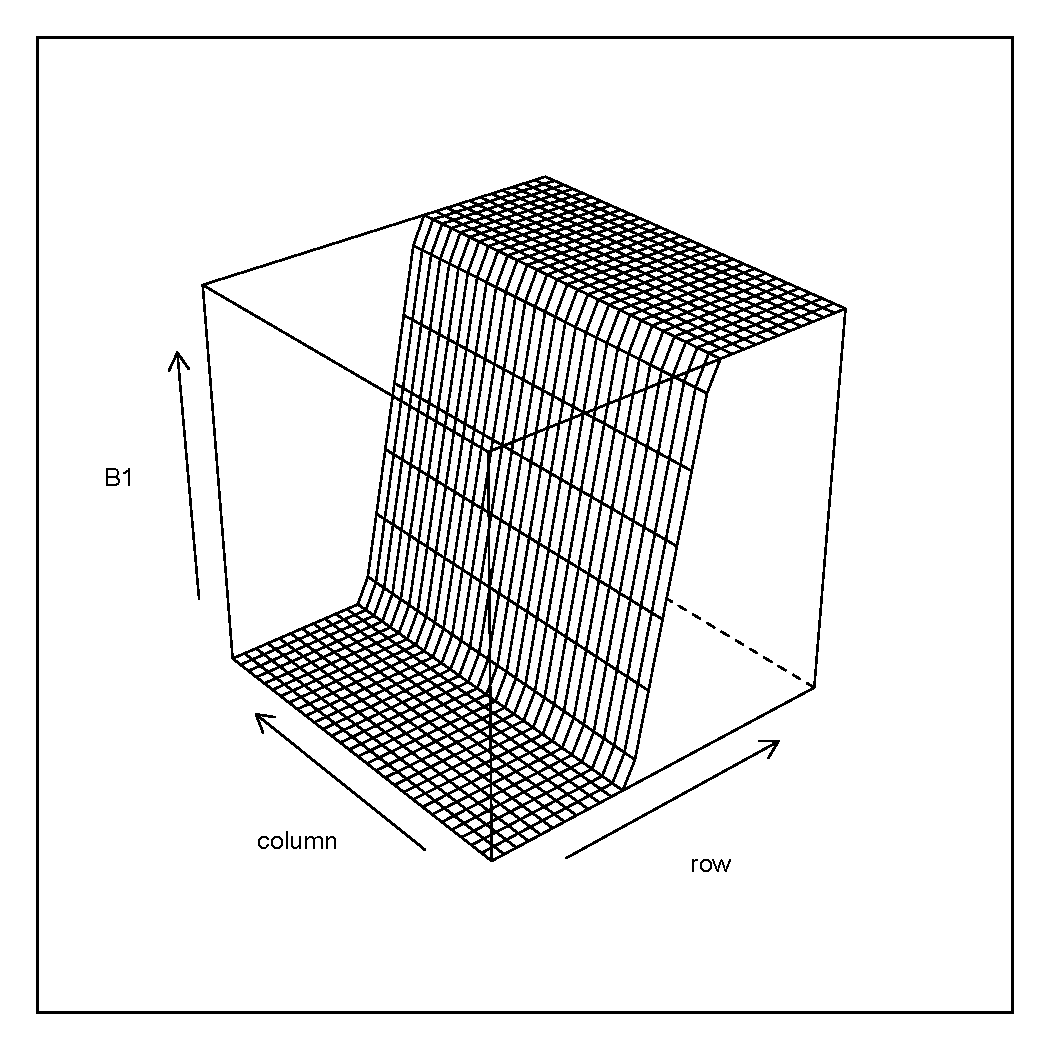
\includegraphics[width=0.32\textwidth]{../../figures/simulation/step.pdf}
			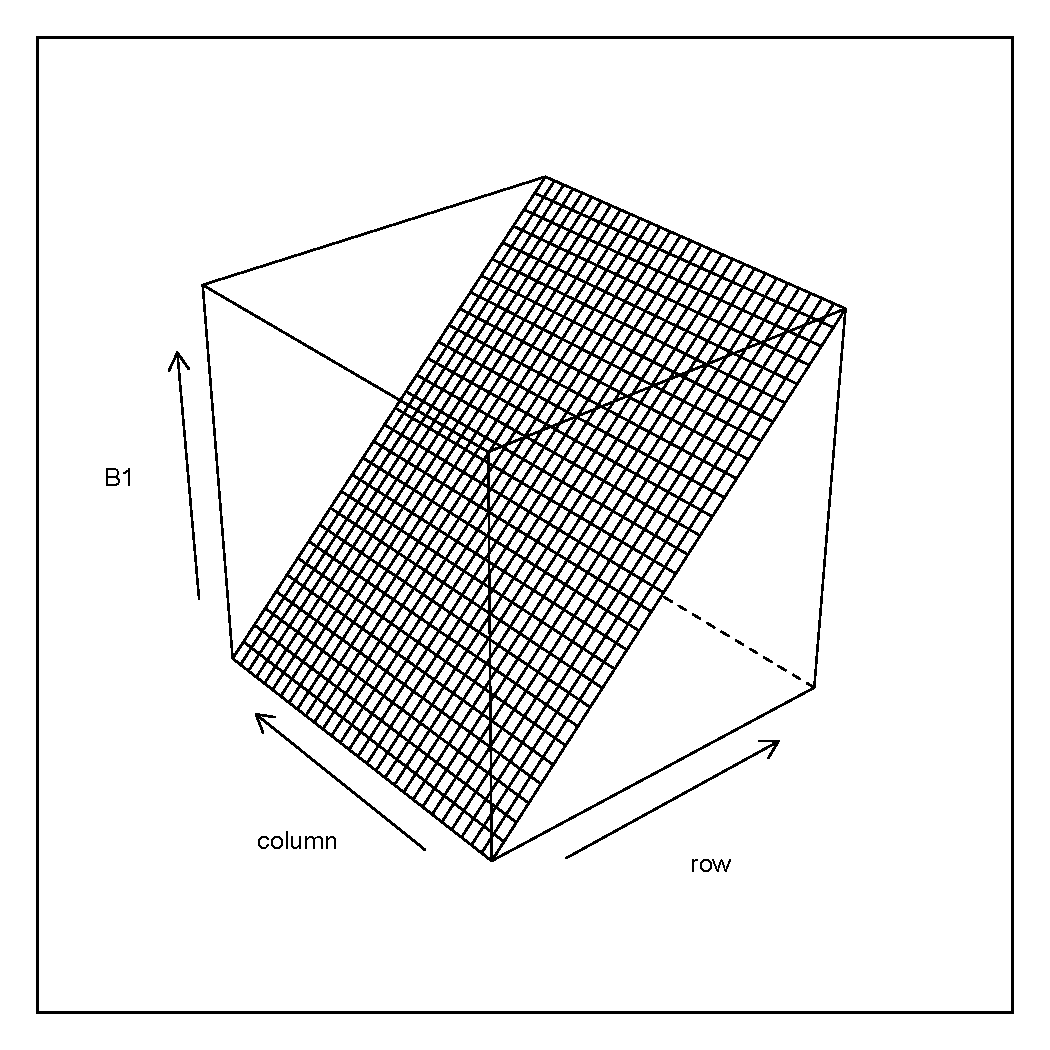
\includegraphics[width=0.32\textwidth]{../../figures/simulation/gradient.pdf}
			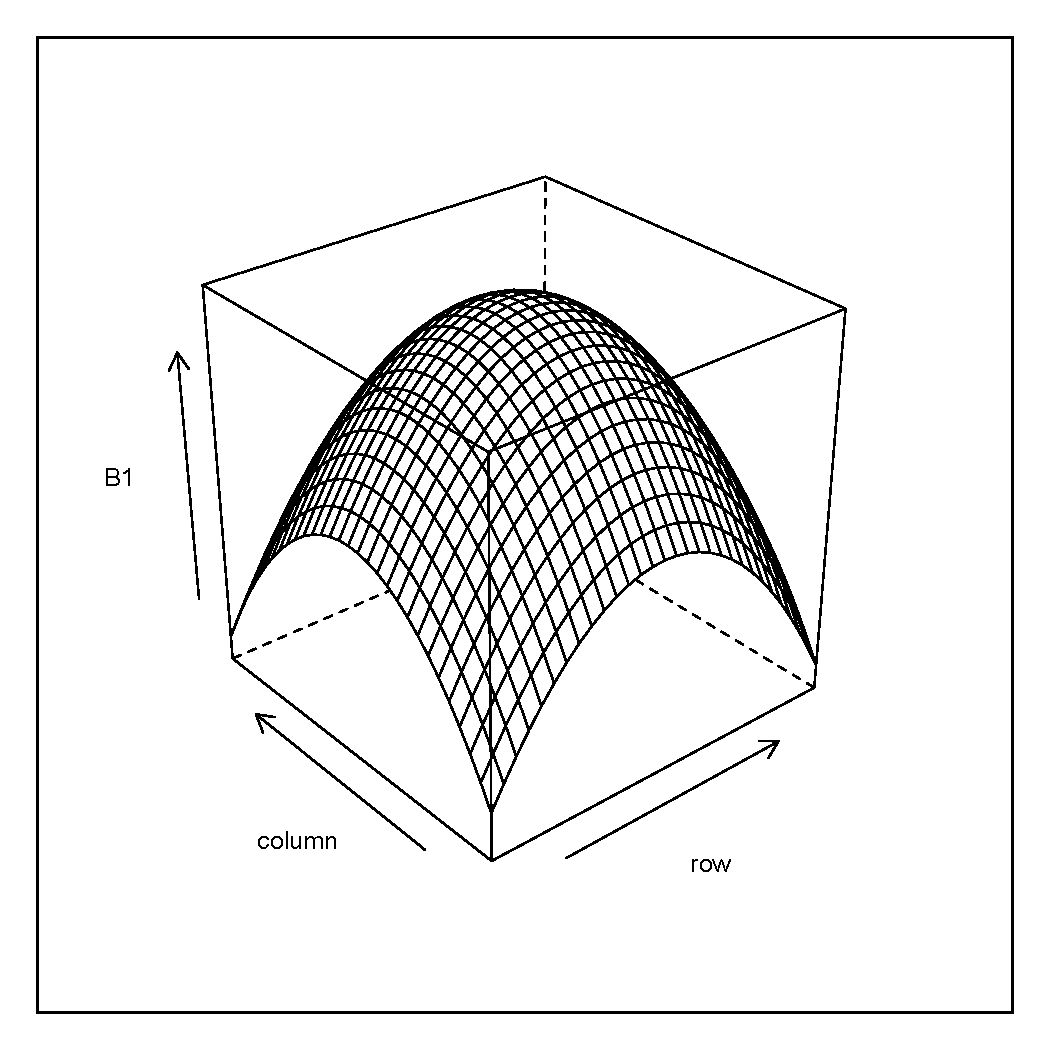
\includegraphics[width=0.32\textwidth]{../../figures/simulation/parabola.pdf}
			\caption{The actual $\beta_1$ coefficient surface used in the simulation.\label{fig:sim-actual}}
		\end{center}
	\end{figure}
	
	\begin{figure}
		\begin{center}
			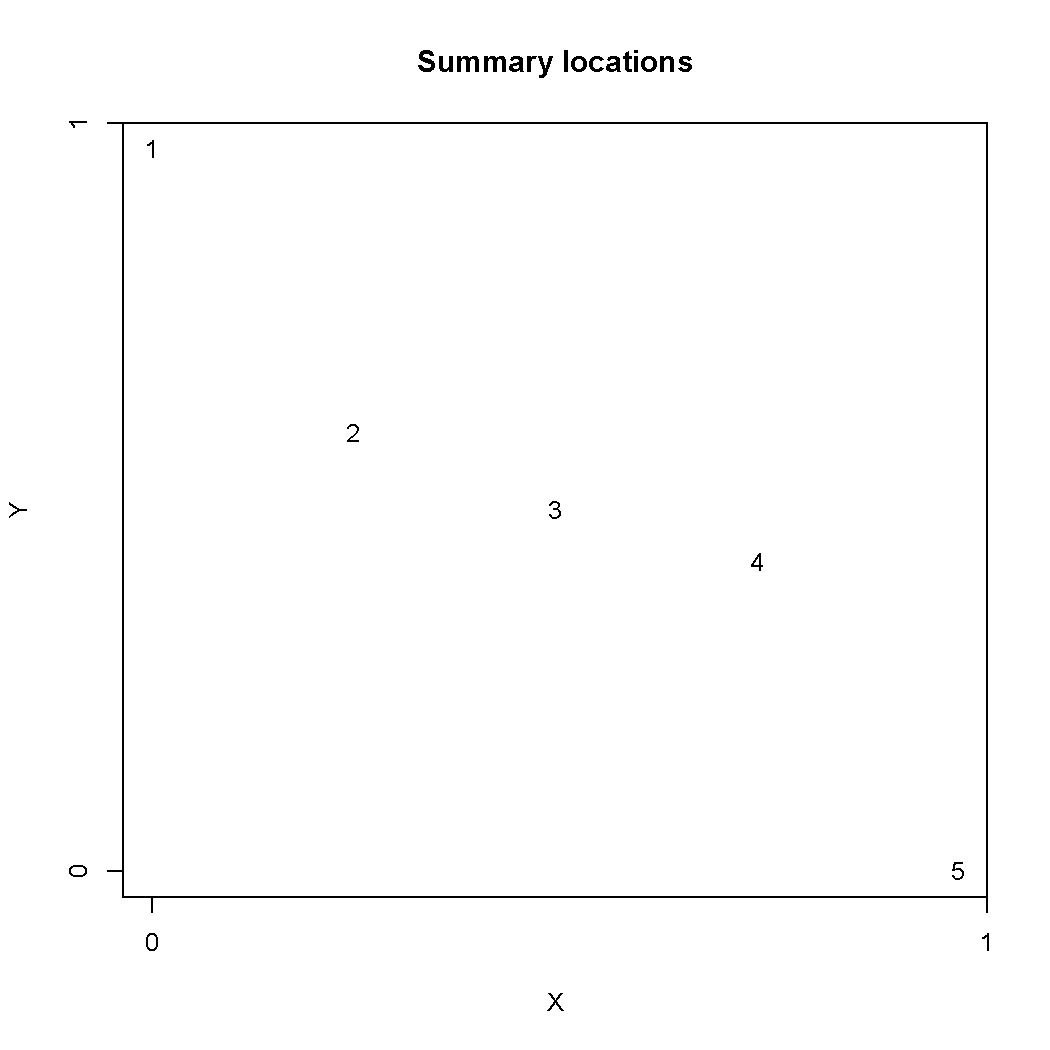
\includegraphics[width=0.5\textwidth]{../../figures/simulation/illustrations/summary-locations.pdf}
			\caption{Locations where the variable selection and coefficient estimation of GWL were summarized.\label{fig:summary-locations}}
		\end{center}
	\end{figure}
	
	\subsection{Results}
	Results from the simulation were summarized at five locations on the simulated grid (see Figure \ref{fig:summary-locations}). The five key locations were chosen because they represent interesting regions of the $\beta_1$ coefficient surfaces. The results of variable selection  and coefficient estimation  are presented in the tables below.\\	
	Selection: Tables \ref{table:loc1-selection} - \ref{table:loc5-selection}\\
	MSE of $\hat{Y}(s_i)$ ($i = 1, \dots, 5$): Tables \ref{table:loc1-MSEY} - \ref{table:loc5-MSEY}\\
	MSE of $\hat{\beta}_1(s_i)$ ($i = 1, \dots, 5$): Tables \ref{table:loc1-X1-MSEX} - \ref{table:loc5-X1-MSEX}\\
	Bias of $\hat{\beta}_1(s_i)$ ($i = 1, \dots, 5$): Tables \ref{table:loc1-X1-BiasX} - \ref{table:loc5-X1-BiasX}\\
	Variance of $\hat{\beta}_1(s_i)$ ($i = 1, \dots, 5$): Tables \ref{table:loc1-X1-varx} - \ref{table:loc5-X1-varx}\\
	
	%Results of the simulation experiment were summarized to asses the consistency in selection and estimation, as well as the coverage properties of the confidence intervals. The confidence intervals based on the bootstrap (without shrinkage) were used for the GWL because they seemed to uniformly outperform the other options.\\ table:loc1-X1-BiasX
	
		
	\subsection{Discussion}
	At locations where $\beta_1$ is nonzero, $X_1$ usually selected for inclusion in all or nearly all of the model runs. An exception is at location four for the step function, where $X_1$ was included in about half of the model runs. This is probably because location four is at the very point where $\beta_1$ transitions from zero to nonzero. Selection performance was relatively poor for the step function at location one, especially for data with $\sigma^2 = 1$. For those simulations, $X_1$ was correctly included in around 85\% of the simulations. The bias, variance, and MSE of $\hat{\beta}_1$ under the same settings were also much larger than the baseline established by the standard \verb!gwr! algorithm. The reason(s) for the poor performance under those particular conditions is currently unknown.\\
	
	Otherwise, selection performance was good, with the rate of false positive selections for $X_2$--$X_5$ (and for $X_1$ where its true coefficient was zero) usually below 0.10. Selection (also bias, variance, and MSE of $\hat{\beta}_1(\bm{s})$) tended to suffer worse by the change from low to high error variance than by the change from low to high collinearity amongst the predictors.\\
	
	There was not a clear and consistent difference in performance between the three selection methods. It might be expected that the adaptive elastic net would outperform the adaptive Lasso under greater covariate collinearity, but if such effect is real it is not apparent from this simulation. The unshrunk coefficient-estimation methods tended to exhibit more bias than the selection-plus-shrinkage methods when the true coefficient value was near zero, and vice versa when the true coefficient was not near zero. The unshrunk methods were perhaps more consistent in their performance and for that reason they are probably preferable in practice.\\
	
	Bias in coefficient estimation was greater and variance less for the standard \verb!gwr! algorithm than for the methods described here. This is probably due to the fact that the methods described here show a preference for smaller bandwidths than those select by \verb!gwr!. Accuracy (as measured by MSE) in fitting the true Y variables was comparable for all the methods. \\	
	
	\subsection{Tables}
		\subsubsection{Selection}
		% latex table generated in R 2.15.2 by xtable 1.7-0 package
		% Thu Apr 18 16:14:00 2013		
		\begin{sidewaystable}
		\begin{center}
		\resizebox{\textheight}{!}{
		\setlength\tabcolsep{4pt}	
		\begin{tabular}{ccc|cc|cc|cc|cc|cc|cc|cc|cc}
		& \multicolumn{6}{c}{\texttt{step}} & \multicolumn{6}{c}{\texttt{gradient}} & \multicolumn{6}{c}{\texttt{parabola}} \\
		location & \multicolumn{2}{c}{\texttt{lars}} & \multicolumn{2}{c}{\texttt{enet}} & \multicolumn{2}{c|}{\texttt{glmnet}} & \multicolumn{2}{c}{\texttt{lars}} & \multicolumn{2}{c}{\texttt{enet}} & \multicolumn{2}{c|}{\texttt{glmnet}}  & \multicolumn{2}{c}{\texttt{lars}} & \multicolumn{2}{c}{\texttt{enet}} & \multicolumn{2}{c}{\texttt{glmnet}}  \\
		& $\beta_1$ & $\beta_4$ - $\beta_5$ & $\beta_1$ & $\beta_4$ - $\beta_5$ & $\beta_1$ & $\beta_4$ - $\beta_5$ & $\beta_1$ & $\beta_4$ - $\beta_5$ & $\beta_1$ & $\beta_4$ - $\beta_5$ & $\beta_1$ & $\beta_4$ - $\beta_5$  & $\beta_1$ & $\beta_4$ - $\beta_5$ & $\beta_1$ & $\beta_4$ - $\beta_5$ & $\beta_1$ & $\beta_4$ - $\beta_5$ \\ 
		  \cline{2-19}
		  \multirow{4}{*}{1}& 0.98 & 0.04 & 1.00 & 0.04 & 1.00 & 0.05 & 1.00 & 0.04 & 1.00 & 0.03 & 1.00 & 0.03 & 0.94 & 0.06 & 0.95 & 0.06 & 0.94 & 0.06 \\ 
		  & 0.89 & 0.09 & 0.86 & 0.09 & 0.82 & 0.07 & 0.99 & 0.08 & 0.97 & 0.07 & 0.97 & 0.07 & 0.80 & 0.06 & 0.81 & 0.07 & 0.80 & 0.06 \\ 
		  & 0.96 & 0.07 & 0.99 & 0.10 & 0.96 & 0.09 & 1.00 & 0.07 & 1.00 & 0.06 & 1.00 & 0.04 & 0.95 & 0.06 & 0.94 & 0.09 & 0.95 & 0.04 \\ 
		  & 0.84 & 0.04 & 0.84 & 0.07 & 0.88 & 0.05 & 0.90 & 0.08 & 0.92 & 0.08 & 0.92 & 0.08 & 0.78 & 0.12 & 0.79 & 0.12 & 0.80 & 0.12\\ 
		  \cline{2-19}
		  \multirow{4}{*}{2} & 1.00 & 0.07 & 1.00 & 0.07 & 1.00 & 0.07 & 1.00 & 0.10 & 1.00 & 0.08 & 1.00 & 0.07 & 1.00 & 0.09 & 1.00 & 0.08 & 1.00 & 0.08 \\ 
		  & 1.00 & 0.06 & 1.00 & 0.06 & 1.00 & 0.07 & 0.98 & 0.07 & 0.98 & 0.08 & 0.99 & 0.07 & 0.97 & 0.12 & 0.98 & 0.11 & 0.98 & 0.10 \\ 
		  & 1.00 & 0.05 & 1.00 & 0.06 & 1.00 & 0.05 & 1.00 & 0.07 & 1.00 & 0.06 & 1.00 & 0.05 & 1.00 & 0.06 & 1.00 & 0.05 & 1.00 & 0.05 \\ 
		  & 0.99 & 0.03 & 1.00 & 0.07 & 0.99 & 0.04 & 0.98 & 0.06 & 0.99 & 0.08 & 0.99 & 0.05 & 0.94 & 0.08 & 0.94 & 0.10 & 0.94 & 0.08 \\ 
		  \cline{2-19}
		  \multirow{4}{*}{3} & 0.99 & 0.05 & 0.99 & 0.06 & 0.99 & 0.06 & 1.00 & 0.09 & 1.00 & 0.08 & 1.00 & 0.07 & 1.00 & 0.09 & 1.00 & 0.09 & 1.00 & 0.09 \\ 
		  & 0.84 & 0.08 & 0.84 & 0.08 & 0.82 & 0.07 & 0.98 & 0.08 & 0.95 & 0.08 & 0.96 & 0.07 & 0.96 & 0.10 & 0.97 & 0.09 & 0.97 & 0.10 \\ 
		  & 0.96 & 0.05 & 0.97 & 0.08 & 0.92 & 0.04 & 1.00 & 0.07 & 1.00 & 0.06 & 1.00 & 0.04 & 1.00 & 0.08 & 1.00 & 0.07 & 1.00 & 0.07 \\ 
		  & 0.78 & 0.08 & 0.81 & 0.11 & 0.80 & 0.08 & 0.93 & 0.09 & 0.95 & 0.09 & 0.94 & 0.09 & 0.93 & 0.10 & 0.94 & 0.10 & 0.96 & 0.10 \\ 
		  \cline{2-19}
		  \multirow{4}{*}{4} & 0.57 & 0.08 & 0.64 & 0.06 & 0.59 & 0.06 & 1.00 & 0.06 & 1.00 & 0.06 & 1.00 & 0.06 & 1.00 & 0.09 & 1.00 & 0.08 & 1.00 & 0.08 \\ 
		  & 0.48 & 0.07 & 0.48 & 0.07 & 0.49 & 0.07 & 0.98 & 0.07 & 0.95 & 0.07 & 0.93 & 0.06 & 0.93 & 0.07 & 0.92 & 0.08 & 0.94 & 0.08 \\ 
		  & 0.45 & 0.08 & 0.51 & 0.12 & 0.40 & 0.07 & 1.00 & 0.09 & 1.00 & 0.08 & 1.00 & 0.10 & 1.00 & 0.08 & 1.00 & 0.08 & 1.00 & 0.08 \\ 
		  & 0.53 & 0.08 & 0.52 & 0.07 & 0.51 & 0.07 & 0.96 & 0.07 & 0.95 & 0.11 & 0.95 & 0.08 & 0.96 & 0.08 & 0.96 & 0.09 & 0.96 & 0.09 \\
		  \cline{2-19}
		  \multirow{4}{*}{5} & 0.04 & 0.03 & 0.03 & 0.03 & 0.03 & 0.03 & 0.92 & 0.05 & 0.93 & 0.05 & 0.94 & 0.04 & 0.93 & 0.10 & 0.93 & 0.09 & 0.92 & 0.10 \\ 
		  & 0.07 & 0.05 & 0.06 & 0.04 & 0.04 & 0.05 & 0.71 & 0.08 & 0.70 & 0.07 & 0.70 & 0.07 & 0.80 & 0.05 & 0.81 & 0.05 & 0.79 & 0.05 \\ 
		  & 0.02 & 0.04 & 0.02 & 0.03 & 0.03 & 0.05 & 0.93 & 0.10 & 0.95 & 0.14 & 0.95 & 0.10 & 0.93 & 0.07 & 0.94 & 0.12 & 0.94 & 0.07 \\ 
		  & 0.05 & 0.04 & 0.04 & 0.03 & 0.06 & 0.06 & 0.60 & 0.07 & 0.63 & 0.13 & 0.64 & 0.06 & 0.81 & 0.09 & 0.81 & 0.11 & 0.83 & 0.08 \\ 
		  \end{tabular}}
		\caption{Selection frequency at location 1\label{table:loc1-selection}}
		\end{center}
		\end{sidewaystable}
		

		\subsubsection{Estimation}
		% latex table generated in R 2.15.2 by xtable 1.7-0 package
		% Thu Apr 18 14:39:33 2013
		%\begin{table}[ht]
		\begin{center}
		\begin{longtable}{cccccccccc}
		  function & location & lars & enet & glmnet & u.lars & u.enet & u.glmnet & oracular & gwr \\ 
		  \hline
		  \multirow{20}{*}{step} & \multirow{4}{*}{1} & 0.046 & 0.025 & \emph{0.023} & 0.151 & 0.127 & 0.124 & 0.082 & \textbf{0.005} \\ 
		  &  & 0.146 & 0.186 & 0.216 & 0.290 & 0.376 & 0.375 & \emph{0.134} & \textbf{0.009} \\ 
		  &  & 0.072 & \emph{0.045} & 0.073 & 0.172 & 0.134 & 0.205 & 0.101 & \textbf{0.011} \\ 
		  &  & 0.214 & 0.218 & 0.179 & 0.441 & 0.425 & 0.369 & \emph{0.154} & \textbf{0.022} \\ 
		  \cline{3-10}
		  & \multirow{4}{*}{2} & 0.024 & 0.024 & 0.024 & \textbf{0.020} & 0.021 & \emph{0.021} & 0.021 & 0.042 \\ 
		  &  & 0.061 & 0.063 & 0.068 & \emph{0.050} & 0.054 & 0.056 & \textbf{0.042} & 0.070 \\ 
		  &  & 0.022 & 0.027 & 0.021 & \textbf{0.017} & 0.021 & \emph{0.017} & 0.018 & 0.044 \\ 
		  &  & 0.069 & 0.071 & 0.071 & 0.057 & \emph{0.056} & 0.061 & \textbf{0.043} & 0.075 \\ 
		  \cline{3-10}
		  & \multirow{4}{*}{3} & 0.011 & 0.011 & 0.010 & 0.007 & 0.007 & 0.007 & \textbf{0.004} & \emph{0.005} \\ 
		  &  & 0.043 & 0.043 & 0.047 & 0.049 & 0.049 & 0.054 & \emph{0.009} & \textbf{0.008} \\ 
		  &  & 0.016 & 0.014 & 0.022 & 0.013 & 0.011 & 0.021 & \textbf{0.005} & \emph{0.005} \\ 
		  &  & 0.048 & 0.047 & 0.045 & 0.049 & 0.045 & 0.044 & \emph{0.008} & \textbf{0.008} \\ 
		  \cline{3-10}
		  & \multirow{4}{*}{4} & \emph{0.014} & 0.014 & \textbf{0.014} & 0.017 & 0.019 & 0.018 & 0.021 & 0.042 \\ 
		  &  & \emph{0.037} & \textbf{0.036} & 0.039 & 0.039 & 0.042 & 0.046 & 0.047 & 0.074 \\ 
		  &  & \textbf{0.010} & 0.012 & \emph{0.011} & 0.013 & 0.016 & 0.014 & 0.020 & 0.044 \\ 
		  &  & \emph{0.038} & \textbf{0.028} & 0.038 & 0.048 & 0.047 & 0.048 & 0.043 & 0.082 \\ 
		  \cline{3-10}
		  & \multirow{4}{*}{5} & 0.002 & \emph{0.001} & 0.002 & 0.006 & 0.004 & 0.004 & \textbf{0.000} & 0.007 \\ 
		  &  & 0.003 & 0.006 & \emph{0.002} & 0.016 & 0.024 & 0.009 & \textbf{0.000} & 0.011 \\ 
		  &  & \emph{0.002} & 0.002 & 0.003 & 0.009 & 0.009 & 0.009 & \textbf{0.000} & 0.010 \\ 
		  &  & 0.017 & \emph{0.004} & 0.022 & 0.046 & 0.038 & 0.043 & \textbf{0.000} & 0.015 \\ 
		  
		  \hline
		  \multirow{20}{*}{gradient} & \multirow{4}{*}{1} & 0.066 & 0.069 & 0.070 & 0.007 & \textbf{0.007} & \emph{0.007} & 0.010 & 0.016 \\ 
		  &  & 0.084 & 0.094 & 0.096 & 0.161 & 0.078 & 0.085 & \emph{0.045} & \textbf{0.042} \\ 
		  &  & 0.065 & 0.070 & 0.069 & 0.009 & \textbf{0.007} & \emph{0.008} & 0.009 & 0.019 \\ 
		  &  & 0.161 & 0.149 & 0.144 & 0.149 & 0.123 & 0.121 & \textbf{0.040} & \emph{0.050} \\ 
		  \cline{3-10}
		  & \multirow{4}{*}{2} & 0.003 & 0.003 & 0.003 & \emph{0.001} & 0.001 & 0.001 & \textbf{0.001} & 0.001 \\ 
		  &  & 0.014 & 0.013 & 0.008 & 0.015 & 0.013 & 0.009 & \emph{0.002} & \textbf{0.002} \\ 
		  &  & 0.003 & 0.003 & 0.003 & 0.001 & \emph{0.001} & \textbf{0.001} & 0.001 & 0.002 \\ 
		  &  & 0.015 & 0.012 & 0.012 & 0.014 & 0.011 & 0.011 & \textbf{0.003} & \emph{0.004} \\ 
		  \cline{3-10}
		  & \multirow{4}{*}{3} & 0.001 & 0.001 & 0.001 & \textbf{0.001} & 0.001 & 0.001 & \emph{0.001} & 0.001 \\ 
		  &  & 0.007 & 0.017 & 0.015 & 0.007 & 0.019 & 0.017 & \emph{0.002} & \textbf{0.002} \\ 
		  &  & 0.001 & 0.001 & 0.000 & 0.000 & \emph{0.000} & \textbf{0.000} & 0.001 & 0.002 \\ 
		  &  & 0.022 & 0.017 & 0.019 & 0.023 & 0.017 & 0.021 & \textbf{0.002} & \emph{0.003} \\ 
		  \cline{3-10}
		  & \multirow{4}{*}{4} & 0.003 & 0.003 & 0.003 & 0.002 & 0.001 & \emph{0.001} & \textbf{0.001} & 0.001 \\ 
		  &  & 0.009 & 0.014 & 0.016 & 0.007 & 0.012 & 0.015 & \textbf{0.002} & \emph{0.003} \\ 
		  &  & 0.003 & 0.002 & 0.003 & 0.002 & 0.001 & \emph{0.001} & \textbf{0.001} & 0.002 \\ 
		  &  & 0.013 & 0.015 & 0.014 & 0.013 & 0.014 & 0.014 & \textbf{0.003} & \emph{0.004} \\ 
		  \cline{3-10}
		  & \multirow{4}{*}{5} & 0.067 & 0.068 & 0.069 & 0.004 & 0.004 & \emph{0.004} & \textbf{0.000} & 0.016 \\ 
		  &  & 0.054 & 0.051 & 0.052 & \emph{0.019} & 0.019 & 0.019 & \textbf{0.000} & 0.044 \\ 
		  &  & 0.062 & 0.060 & 0.064 & 0.009 & 0.010 & \emph{0.007} & \textbf{0.000} & 0.021 \\ 
		  &  & 0.050 & 0.047 & 0.053 & \emph{0.017} & 0.020 & 0.017 & \textbf{0.000} & 0.051 \\ 

		  \pagebreak
		  \multirow{20}{*}{parabola} & \multirow{4}{*}{1} & 0.074 & 0.075 & 0.074 & 0.020 & \emph{0.020} & \textbf{0.020} & 0.022 & 0.105 \\ 
		  &  & 0.079 & 0.078 & 0.077 & 0.041 & \emph{0.040} & \textbf{0.039} & 0.063 & 0.106 \\ 
		  &  & 0.077 & 0.069 & 0.076 & 0.024 & \textbf{0.018} & 0.023 & \emph{0.023} & 0.099 \\ 
		  &  & 0.083 & 0.072 & 0.083 & \emph{0.048} & \textbf{0.044} & 0.050 & 0.067 & 0.110 \\ 
		  \cline{3-10}
		  & \multirow{4}{*}{2} & \emph{0.005} & 0.005 & 0.005 & 0.007 & 0.007 & 0.007 & \textbf{0.004} & 0.007 \\ 
		  &  & 0.018 & 0.016 & 0.016 & 0.026 & 0.021 & 0.022 & \emph{0.008} & \textbf{0.007} \\ 
		  &  & 0.007 & 0.007 & \emph{0.007} & 0.011 & 0.010 & 0.009 & \textbf{0.004} & 0.008 \\ 
		  &  & 0.020 & 0.022 & 0.020 & 0.022 & 0.022 & 0.023 & \textbf{0.007} & \emph{0.009} \\ 
		  \cline{3-10}
		  & \multirow{4}{*}{3} & 0.015 & 0.015 & 0.015 & 0.015 & 0.015 & \emph{0.015} & \textbf{0.005} & 0.022 \\ 
		  &  & 0.032 & 0.029 & 0.029 & 0.030 & 0.027 & 0.027 & \textbf{0.012} & \emph{0.023} \\ 
		  &  & 0.019 & 0.018 & 0.019 & 0.018 & \emph{0.017} & 0.018 & \textbf{0.005} & 0.024 \\ 
		  &  & 0.037 & 0.037 & 0.030 & 0.037 & 0.034 & 0.029 & \textbf{0.012} & \emph{0.024} \\ 
		  \cline{3-10}
		  & \multirow{4}{*}{4} & 0.006 & 0.006 & \emph{0.006} & 0.009 & 0.009 & 0.009 & \textbf{0.004} & 0.008 \\ 
		  &  & 0.025 & 0.027 & 0.023 & 0.027 & 0.029 & 0.024 & \emph{0.010} & \textbf{0.009} \\ 
		  &  & \emph{0.008} & 0.008 & 0.008 & 0.011 & 0.011 & 0.011 & \textbf{0.004} & 0.010 \\ 
		  &  & 0.018 & 0.020 & 0.017 & 0.022 & 0.022 & 0.022 & \textbf{0.009} & \emph{0.010} \\ 
		  \cline{3-10}
		  & \multirow{4}{*}{5} & 0.074 & 0.075 & 0.075 & \textbf{0.018} & 0.020 & 0.021 & \emph{0.020} & 0.104 \\ 
		  &  & 0.075 & 0.074 & 0.073 & 0.024 & \textbf{0.022} & \emph{0.023} & 0.055 & 0.104 \\ 
		  &  & 0.077 & 0.069 & 0.076 & \emph{0.021} & 0.023 & \textbf{0.020} & 0.025 & 0.099 \\ 
		  &  & 0.081 & 0.075 & 0.081 & 0.037 & \emph{0.036} & \textbf{0.035} & 0.042 & 0.113 \\ 		  
		\caption{Mean squared error of estimates for $\beta_1$ (\textbf{minimum}, \emph{next best}).\label{table:X1-MSEX}}
		\end{longtable}
		\end{center}
		%\end{table}	
 
 % latex table generated in R 2.15.2 by xtable 1.7-0 package
		% Thu Apr 18 14:39:33 2013
		%\begin{longtable}
		\begin{center}
		\begin{longtable}{cccccccccc}
		  function & location & lars & enet & glmnet & u.lars & u.enet & u.glmnet & oracular & gwr \\ 
		  \hline
		  \multirow{20}{*}{step} & \multirow{4}{*}{1} & -0.057 & -0.029 & -0.020 & \textbf{-0.003} & 0.038 & 0.033 & 0.034 & \emph{-0.004} \\ 
&  & -0.150 & -0.195 & -0.211 & \textbf{-0.004} & -0.082 & -0.075 & 0.053 & \emph{-0.017} \\ 
&  & -0.090 & -0.077 & -0.073 & \textbf{0.002} & 0.028 & \emph{-0.014} & 0.050 & -0.017 \\ 
&  & -0.208 & -0.214 & -0.167 & -0.053 & -0.067 & -0.068 & \emph{0.035} & \textbf{0.006} \\ 
		  \cline{3-10}
		  & \multirow{4}{*}{2} & -0.117 & -0.119 & -0.119 & \textbf{-0.106} & -0.110 & \emph{-0.110} & -0.124 & -0.196 \\ 
&  & -0.178 & -0.178 & -0.186 & \emph{-0.145} & \textbf{-0.145} & -0.150 & -0.175 & -0.253 \\ 
&  & -0.103 & -0.130 & -0.099 & \textbf{-0.083} & -0.103 & \emph{-0.083} & -0.110 & -0.199 \\ 
&  & -0.212 & -0.221 & -0.216 & \emph{-0.175} & \textbf{-0.167} & -0.184 & -0.182 & -0.263 \\
		  \cline{3-10}
		  & \multirow{4}{*}{3} & -0.014 & \emph{-0.014} & \textbf{-0.010} & 0.018 & 0.017 & 0.015 & 0.021 & 0.040 \\ 
&  & -0.026 & -0.027 & -0.031 & \emph{0.006} & 0.009 & \textbf{0.004} & 0.050 & 0.059 \\ 
&  & -0.044 & -0.056 & -0.056 & \emph{-0.013} & \textbf{-0.009} & -0.030 & 0.017 & 0.034 \\ 
&  & -0.083 & -0.094 & -0.077 & -0.059 & -0.056 & -0.056 & \textbf{0.017} & \emph{0.055} \\ 
		  \cline{3-10}
		  & \multirow{4}{*}{4} & \textbf{0.047} & 0.059 & \emph{0.049} & 0.058 & 0.074 & 0.065 & 0.129 & 0.196 \\ 
&  & \textbf{0.072} & \emph{0.075} & 0.076 & 0.080 & 0.088 & 0.090 & 0.193 & 0.263 \\ 
&  & \emph{0.014} & 0.027 & \textbf{0.010} & 0.027 & 0.043 & 0.020 & 0.129 & 0.199 \\ 
&  & 0.091 & \textbf{0.073} & \emph{0.089} & 0.108 & 0.105 & 0.105 & 0.189 & 0.275 \\ 
		  \cline{3-10}
		  & \multirow{4}{*}{5} & -0.009 & \emph{-0.006} & -0.006 & -0.015 & -0.009 & -0.010 & \textbf{0.000} & -0.006 \\ 
&  & 0.001 & -0.009 & \emph{-0.000} & -0.018 & -0.025 & -0.008 & \textbf{0.000} & -0.011 \\ 
&  & -0.006 & \emph{-0.005} & -0.009 & -0.010 & -0.009 & -0.012 & \textbf{0.000} & -0.009 \\ 
&  & -0.012 & -0.011 & -0.011 & -0.026 & -0.036 & -0.021 & \textbf{0.000} & \emph{-0.007} \\ 
		  \hline
		  \multirow{20}{*}{gradient} & \multirow{4}{*}{1} & -0.246 & -0.248 & -0.253 & \textbf{0.008} & \emph{0.010} & 0.011 & 0.011 & -0.111 \\ 
&  & -0.233 & -0.242 & -0.248 & 0.026 & \emph{-0.014} & -0.022 & \textbf{-0.007} & -0.182 \\ 
&  & -0.245 & -0.259 & -0.255 & -0.004 & \emph{-0.003} & \textbf{-0.000} & 0.003 & -0.112 \\ 
&  & -0.306 & -0.290 & -0.287 & -0.083 & \emph{-0.055} & -0.080 & \textbf{0.017} & -0.197 \\ 
		  \cline{3-10}
		  & \multirow{4}{*}{2} & -0.046 & -0.047 & -0.048 & \textbf{0.000} & 0.002 & \emph{0.001} & 0.004 & 0.002 \\ 
&  & -0.034 & -0.044 & -0.035 & 0.009 & \textbf{0.003} & 0.011 & \emph{0.008} & -0.011 \\ 
&  & -0.039 & -0.046 & -0.043 & 0.003 & 0.003 & 0.003 & \textbf{0.002} & \emph{0.002} \\ 
&  & -0.058 & -0.062 & -0.056 & -0.016 & -0.011 & \emph{-0.009} & \textbf{-0.002} & -0.020 \\
		  \cline{3-10}
		  & \multirow{4}{*}{3} & 0.007 & 0.005 & 0.005 & 0.003 & \emph{0.002} & \textbf{0.001} & 0.003 & 0.002 \\ 
&  & -0.004 & -0.017 & -0.012 & \textbf{-0.003} & -0.013 & -0.007 & \emph{0.003} & 0.006 \\ 
&  & 0.006 & 0.005 & 0.006 & 0.001 & \emph{0.000} & 0.000 & 0.003 & \textbf{0.000} \\ 
&  & -0.019 & -0.029 & -0.018 & -0.012 & -0.022 & -0.013 & \textbf{-0.002} & \emph{0.003} \\ 
		  \cline{3-10}
		  & \multirow{4}{*}{4} & 0.047 & 0.043 & 0.045 & 0.009 & \emph{0.006} & 0.007 & \textbf{0.004} & 0.008 \\ 
&  & 0.021 & 0.006 & \textbf{0.002} & \emph{-0.003} & -0.014 & -0.023 & 0.004 & 0.020 \\ 
&  & 0.039 & 0.038 & 0.039 & \emph{0.001} & -0.001 & -0.001 & \textbf{0.000} & -0.001 \\ 
&  & \textbf{0.000} & -0.009 & 0.003 & -0.009 & -0.021 & -0.013 & \emph{-0.003} & 0.014 \\ 
		  \cline{3-10}
		  & \multirow{4}{*}{5} & 0.246 & 0.249 & 0.253 & 0.002 & \emph{0.002} & 0.003 & \textbf{0.000} & 0.113 \\ 
&  & 0.191 & 0.182 & 0.186 & 0.007 & \emph{-0.001} & 0.004 & \textbf{0.000} & 0.187 \\ 
&  & 0.234 & 0.234 & 0.243 & 0.007 & \emph{-0.001} & 0.008 & \textbf{0.000} & 0.115 \\ 
&  & 0.168 & 0.165 & 0.179 & 0.030 & \emph{0.024} & 0.029 & \textbf{0.000} & 0.190 \\ 
		  \pagebreak	  
		  \multirow{20}{*}{parabola} & \multirow{4}{*}{1} & 0.252 & 0.254 & 0.252 & 0.091 & 0.090 & \emph{0.090} & \textbf{0.029} & 0.323 \\ 
&  & 0.240 & 0.241 & 0.236 & 0.130 & 0.129 & \emph{0.126} & \textbf{0.070} & 0.322 \\ 
&  & 0.262 & 0.245 & 0.259 & 0.091 & \emph{0.083} & 0.101 & \textbf{0.041} & 0.313 \\ 
&  & 0.239 & 0.222 & 0.242 & 0.121 & \emph{0.095} & 0.115 & \textbf{0.068} & 0.323 \\ 
		  \cline{3-10}
		  & \multirow{4}{*}{2} & -0.062 & -0.063 & \emph{-0.062} & -0.073 & -0.074 & -0.072 & \textbf{-0.048} & -0.079 \\ 
&  & -0.067 & -0.066 & \textbf{-0.063} & -0.069 & -0.068 & \emph{-0.065} & -0.072 & -0.078 \\ 
&  & \emph{-0.073} & -0.079 & -0.076 & -0.087 & -0.091 & -0.087 & \textbf{-0.052} & -0.085 \\ 
&  & -0.093 & -0.104 & -0.097 & -0.101 & -0.102 & -0.101 & \textbf{-0.065} & \emph{-0.078} \\
		  \cline{3-10}
		  & \multirow{4}{*}{3} & -0.107 & -0.107 & -0.106 & -0.103 & -0.103 & \emph{-0.102} & \textbf{-0.057} & -0.148 \\ 
&  & -0.141 & -0.136 & -0.132 & -0.129 & -0.122 & \emph{-0.121} & \textbf{-0.090} & -0.147 \\ 
&  & -0.125 & -0.127 & -0.125 & -0.123 & \emph{-0.121} & -0.121 & \textbf{-0.060} & -0.154 \\ 
&  & -0.147 & -0.156 & -0.131 & -0.137 & -0.136 & \emph{-0.121} & \textbf{-0.092} & -0.147 \\ 
		  \cline{3-10}
		  & \multirow{4}{*}{4} & \emph{-0.066} & -0.070 & -0.069 & -0.078 & -0.083 & -0.081 & \textbf{-0.051} & -0.088 \\ 
&  & -0.113 & -0.119 & -0.110 & -0.119 & -0.126 & -0.115 & \textbf{-0.081} & \emph{-0.088} \\ 
&  & -0.080 & -0.085 & \emph{-0.078} & -0.092 & -0.095 & -0.090 & \textbf{-0.055} & -0.095 \\ 
&  & -0.088 & -0.099 & -0.088 & -0.094 & -0.099 & -0.094 & \textbf{-0.079} & \emph{-0.086} \\ 
		  \cline{3-10}
		  & \multirow{4}{*}{5} & 0.253 & 0.256 & 0.253 & \emph{0.085} & 0.091 & 0.089 & \textbf{0.022} & 0.321 \\ 
&  & 0.234 & 0.233 & 0.228 & 0.095 & \emph{0.088} & 0.089 & \textbf{0.004} & 0.319 \\ 
&  & 0.257 & 0.243 & 0.257 & 0.093 & \emph{0.079} & 0.088 & \textbf{0.052} & 0.313 \\ 
&  & 0.243 & 0.232 & 0.246 & 0.120 & \emph{0.096} & 0.110 & \textbf{0.069} & 0.328 \\ 
		
		\caption{Bias of estimates for $\beta_1$ (\textbf{minimum}, \emph{next best}).\label{table:X1-bias}}
		\end{longtable}
		\end{center}
		%\end{longtable}	
		%\end{comment}

		
		
% latex table generated in R 2.15.2 by xtable 1.7-0 package
% Wed May  1 20:51:29 2013
%\begin{table}[ht]
\begin{center}
\begin{longtable}{cccccccccc}
  function & location & lars & enet & glmnet & u.lars & u.enet & u.glmnet & oracular & gwr \\ 
  \hline
   \multirow{20}{*}{step} & \multirow{4}{*}{1} & 0.043 & 0.024 & \emph{0.023} & 0.152 & 0.127 & 0.124 & 0.081 & \textbf{0.005} \\ 
  &  & \emph{0.125} & 0.149 & 0.173 & 0.293 & 0.373 & 0.373 & 0.133 & \textbf{0.009} \\ 
  &  & 0.064 & \emph{0.040} & 0.068 & 0.173 & 0.134 & 0.207 & 0.099 & \textbf{0.011} \\ 
  &  & 0.173 & 0.174 & \emph{0.153} & 0.443 & 0.424 & 0.368 & 0.154 & \textbf{0.022} \\ 
  \cline{3-10}
  & \multirow{4}{*}{2} & 0.010 & 0.010 & 0.010 & 0.009 & 0.009 & 0.009 & \emph{0.006} & \textbf{0.003} \\ 
  &  & 0.029 & 0.032 & 0.034 & 0.029 & 0.033 & 0.034 & \emph{0.012} & \textbf{0.006} \\ 
  &  & 0.011 & 0.011 & 0.012 & 0.010 & 0.010 & 0.010 & \emph{0.006} & \textbf{0.005} \\ 
  &  & 0.024 & 0.022 & 0.025 & 0.026 & 0.028 & 0.028 & \emph{0.010} & \textbf{0.006} \\ 
  \cline{3-10}
  & \multirow{4}{*}{3} & 0.011 & 0.011 & 0.010 & 0.007 & 0.007 & 0.007 & \emph{0.004} & \textbf{0.003} \\ 
  &  & 0.043 & 0.043 & 0.047 & 0.050 & 0.050 & 0.055 & \emph{0.007} & \textbf{0.004} \\ 
  &  & 0.014 & 0.011 & 0.019 & 0.013 & 0.011 & 0.020 & \emph{0.004} & \textbf{0.004} \\ 
  &  & 0.041 & 0.039 & 0.039 & 0.046 & 0.043 & 0.042 & \emph{0.008} & \textbf{0.005} \\ 
  \cline{3-10}
  & \multirow{4}{*}{4} & 0.012 & 0.011 & 0.012 & 0.014 & 0.014 & 0.014 & \emph{0.004} & \textbf{0.003} \\ 
  &  & 0.032 & 0.030 & 0.033 & 0.033 & 0.035 & 0.038 & \emph{0.009} & \textbf{0.005} \\ 
  &  & 0.010 & 0.011 & 0.011 & 0.013 & 0.014 & 0.013 & \textbf{0.003} & \emph{0.004} \\ 
  &  & 0.029 & 0.023 & 0.031 & 0.037 & 0.037 & 0.037 & \emph{0.007} & \textbf{0.006} \\ 
  \cline{3-10}
  & \multirow{4}{*}{5} & 0.002 & \emph{0.001} & 0.002 & 0.006 & 0.004 & 0.004 & \textbf{0.000} & 0.007 \\ 
  &  & 0.003 & 0.006 & \emph{0.002} & 0.016 & 0.024 & 0.009 & \textbf{0.000} & 0.011 \\ 
  &  & \emph{0.002} & 0.002 & 0.003 & 0.009 & 0.009 & 0.009 & \textbf{0.000} & 0.010 \\ 
  &  & 0.017 & \emph{0.004} & 0.022 & 0.045 & 0.037 & 0.043 & \textbf{0.000} & 0.015 \\ 
  \hline
  
  \multirow{20}{*}{gradient} & \multirow{4}{*}{1} & \emph{0.001} & 0.001 & 0.001 & 0.001 & 0.001 & 0.001 & \textbf{0.001} & 0.001 \\ 
  &  & 0.013 & 0.011 & 0.007 & 0.016 & 0.013 & 0.009 & \emph{0.002} & \textbf{0.002} \\ 
  &  & 0.001 & \emph{0.001} & 0.001 & 0.001 & 0.001 & \textbf{0.001} & 0.001 & 0.002 \\ 
  &  & 0.011 & 0.008 & 0.009 & 0.014 & 0.011 & 0.011 & \textbf{0.003} & \emph{0.003} \\ 
  \cline{3-10}  
  & \multirow{4}{*}{2} & \emph{0.006} & 0.007 & 0.006 & 0.008 & 0.007 & 0.007 & 0.010 & \textbf{0.004} \\ 
  &  & \emph{0.030} & 0.035 & 0.035 & 0.162 & 0.079 & 0.085 & 0.046 & \textbf{0.009} \\ 
  &  & 0.005 & \textbf{0.003} & \emph{0.004} & 0.009 & 0.007 & 0.008 & 0.009 & 0.007 \\ 
  &  & 0.068 & 0.066 & 0.062 & 0.143 & 0.121 & 0.116 & \emph{0.040} & \textbf{0.011} \\ 
  \cline{3-10}
  & \multirow{4}{*}{3} & 0.001 & 0.001 & 0.001 & \textbf{0.001} & 0.001 & 0.001 & \emph{0.001} & 0.001 \\ 
  &  & 0.007 & 0.017 & 0.015 & 0.007 & 0.019 & 0.017 & \emph{0.002} & \textbf{0.002} \\ 
  &  & 0.001 & 0.001 & 0.000 & 0.000 & \emph{0.000} & \textbf{0.000} & 0.001 & 0.002 \\ 
  &  & 0.022 & 0.016 & 0.019 & 0.023 & 0.016 & 0.021 & \textbf{0.002} & \emph{0.003} \\ 
  \cline{3-10}
  & \multirow{4}{*}{4} & 0.001 & 0.001 & 0.001 & 0.002 & 0.001 & \emph{0.001} & \textbf{0.001} & 0.001 \\ 
  &  & 0.008 & 0.014 & 0.017 & 0.007 & 0.012 & 0.014 & \textbf{0.002} & \emph{0.002} \\ 
  &  & 0.001 & 0.001 & 0.001 & 0.002 & 0.001 & \emph{0.001} & \textbf{0.001} & 0.002 \\ 
  &  & 0.013 & 0.015 & 0.014 & 0.013 & 0.014 & 0.014 & \textbf{0.003} & \emph{0.004} \\ 
  \cline{3-10}
  & \multirow{4}{*}{5} & 0.007 & 0.006 & 0.005 & 0.004 & 0.004 & 0.004 & \textbf{0.000} & \emph{0.003} \\ 
  &  & 0.018 & 0.018 & 0.018 & 0.019 & 0.020 & 0.020 & \textbf{0.000} & \emph{0.009} \\ 
  &  & 0.007 & 0.005 & \emph{0.005} & 0.009 & 0.010 & 0.007 & \textbf{0.000} & 0.008 \\ 
  &  & 0.022 & 0.020 & 0.021 & 0.016 & 0.020 & 0.016 & \textbf{0.000} & \emph{0.015} \\ 
  \pagebreak
  
  \multirow{20}{*}{parabola} & \multirow{4}{*}{1} & 0.010 & \emph{0.010} & 0.010 & 0.012 & 0.012 & 0.012 & 0.022 & \textbf{0.001} \\ 
  &  & 0.021 & \emph{0.020} & 0.021 & 0.024 & 0.024 & 0.024 & 0.058 & \textbf{0.002} \\ 
  &  & \emph{0.009} & 0.009 & 0.009 & 0.015 & 0.011 & 0.013 & 0.021 & \textbf{0.001} \\ 
  &  & 0.026 & \emph{0.023} & 0.025 & 0.034 & 0.035 & 0.037 & 0.064 & \textbf{0.006} \\ 
  \cline{3-10}
  & \multirow{4}{*}{2} & \emph{0.001} & 0.001 & 0.001 & 0.002 & 0.002 & 0.002 & 0.001 & \textbf{0.000} \\ 
  &  & 0.014 & 0.012 & 0.012 & 0.021 & 0.017 & 0.018 & \emph{0.003} & \textbf{0.001} \\ 
  &  & 0.001 & 0.001 & \emph{0.001} & 0.003 & 0.002 & 0.002 & 0.001 & \textbf{0.000} \\ 
  &  & 0.012 & 0.011 & 0.011 & 0.012 & 0.012 & 0.013 & \emph{0.003} & \textbf{0.003} \\ 
  \cline{3-10}
  & \multirow{4}{*}{3} & 0.004 & 0.004 & 0.004 & 0.005 & 0.005 & 0.005 & \emph{0.002} & \textbf{0.000} \\ 
  &  & 0.012 & 0.010 & 0.012 & 0.014 & 0.013 & 0.013 & \emph{0.004} & \textbf{0.001} \\ 
  &  & 0.003 & 0.002 & 0.003 & 0.003 & 0.003 & 0.003 & \emph{0.002} & \textbf{0.000} \\ 
  &  & 0.016 & 0.013 & 0.013 & 0.018 & 0.016 & 0.015 & \emph{0.004} & \textbf{0.002} \\ 
  \cline{3-10}
  & \multirow{4}{*}{4} & 0.002 & \emph{0.001} & 0.001 & 0.003 & 0.002 & 0.002 & 0.001 & \textbf{0.000} \\ 
  &  & 0.012 & 0.013 & 0.011 & 0.013 & 0.013 & 0.011 & \emph{0.003} & \textbf{0.001} \\ 
  &  & 0.001 & \emph{0.001} & 0.002 & 0.003 & 0.001 & 0.003 & 0.001 & \textbf{0.001} \\ 
  &  & 0.011 & 0.010 & 0.010 & 0.014 & 0.012 & 0.013 & \emph{0.003} & \textbf{0.003} \\ 
  \cline{3-10}
  & \multirow{4}{*}{5} & 0.010 & \emph{0.010} & 0.011 & 0.011 & 0.012 & 0.013 & 0.019 & \textbf{0.001} \\ 
  &  & 0.021 & 0.019 & 0.021 & 0.016 & \emph{0.014} & 0.015 & 0.056 & \textbf{0.003} \\ 
  &  & 0.011 & 0.010 & \emph{0.010} & 0.013 & 0.017 & 0.012 & 0.023 & \textbf{0.001} \\ 
  &  & 0.022 & 0.021 & \emph{0.021} & 0.023 & 0.027 & 0.023 & 0.038 & \textbf{0.005} \\   
\caption{Variance of estimates for $\beta_1$ (\textbf{minimum}, \emph{next best}).\label{table:X1-varx}}
\end{longtable}
\end{center}



% latex table generated in R 2.15.2 by xtable 1.7-0 package
% Wed May  1 20:56:30 2013
\begin{table}[ht]
\begin{center}
\begin{tabular}{ccccccccc}
  & lars & enet & glmnet & u.lars & u.enet & u.glmnet & oracular & gwr \\ 
  \cline{2-9}
  \multirow{4}{*}{step} & 0.130 & \textbf{0.100} & 0.101 & 0.130 & \emph{0.100} & 0.101 & 0.111 & 0.118 \\ 
  & \textbf{0.483} & 0.594 & 0.564 & \emph{0.483} & 0.594 & 0.564 & 0.694 & 0.850 \\ 
  & 0.196 & \emph{0.151} & 0.169 & 0.196 & \textbf{0.151} & 0.169 & 0.213 & 0.247 \\ 
  & 0.563 & 0.559 & \textbf{0.552} & 0.563 & 0.559 & \emph{0.552} & 0.757 & 0.895 \\ 
  \cline{2-9}
  \multirow{4}{*}{gradient} & 0.235 & 0.224 & 0.232 & 0.235 & 0.224 & 0.232 & \emph{0.223} & \textbf{0.222} \\ 
  & 0.693 & \textbf{0.669} & 0.671 & 0.693 & \emph{0.669} & 0.671 & 0.723 & 0.757 \\ 
  & 0.257 & 0.258 & 0.260 & 0.257 & 0.258 & 0.260 & \emph{0.237} & \textbf{0.210} \\ 
  & \textbf{0.724} & 0.733 & 0.731 & \emph{0.724} & 0.733 & 0.731 & 0.815 & 0.784 \\ 
  \cline{2-9}
  \multirow{4}{*}{parabola} & 0.145 & 0.142 & \textbf{0.140} & 0.145 & 0.142 & \emph{0.140} & 0.157 & 0.248 \\ 
  & 1.275 & \emph{1.257} & 1.266 & 1.275 & 1.257 & 1.266 & \textbf{1.153} & 1.466 \\ 
  & 0.299 & \emph{0.285} & 0.295 & 0.299 & 0.285 & 0.295 & \textbf{0.270} & 0.434 \\ 
  & 0.835 & \textbf{0.801} & 0.806 & 0.835 & \emph{0.801} & 0.806 & 0.862 & 0.986 \\ 
  \end{tabular}
\caption{Mean squared error of estimates for $Y$ at location 1 (\textbf{minimum}, \emph{next best}).\label{table:loc1-MSEY}}
\end{center}
\end{table}
% latex table generated in R 2.15.2 by xtable 1.7-0 package
% Wed May  1 20:56:30 2013
\begin{table}[ht]
\begin{center}
\begin{tabular}{ccccccccc}
  & lars & enet & glmnet & u.lars & u.enet & u.glmnet & oracular & gwr \\ 
  \cline{2-9}
  \multirow{4}{*}{step} & \textbf{0.193} & 0.196 & 0.194 & \emph{0.193} & 0.196 & 0.194 & 0.225 & 0.244 \\ 
  & 1.023 & 1.019 & \textbf{1.001} & 1.023 & 1.019 & \emph{1.001} & 1.171 & 1.123 \\ 
  & \textbf{0.270} & 0.275 & 0.273 & \emph{0.270} & 0.275 & 0.273 & 0.311 & 0.332 \\ 
  & 0.973 & \textbf{0.897} & 0.953 & 0.973 & \emph{0.897} & 0.953 & 1.000 & 1.048 \\ 
  \cline{2-9}
  \multirow{4}{*}{gradient} & 0.218 & 0.216 & 0.218 & 0.218 & \emph{0.216} & 0.218 & 0.221 & \textbf{0.210} \\ 
  & 0.828 & \textbf{0.814} & 0.836 & 0.828 & \emph{0.814} & 0.836 & 0.863 & 0.832 \\ 
  & 0.257 & 0.257 & 0.257 & 0.257 & 0.257 & 0.257 & \emph{0.257} & \textbf{0.247} \\ 
  & \textbf{0.795} & 0.819 & 0.803 & \emph{0.795} & 0.819 & 0.803 & 0.822 & 0.799 \\ 
  \cline{2-9}
  \multirow{4}{*}{parabola} & \emph{0.192} & 0.195 & 0.193 & \textbf{0.192} & 0.195 & 0.193 & 0.204 & 0.199 \\ 
  & \textbf{1.139} & 1.193 & 1.152 & \emph{1.139} & 1.193 & 1.152 & 1.204 & 1.214 \\ 
  & \emph{0.248} & 0.254 & 0.250 & 0.248 & 0.254 & 0.250 & \textbf{0.246} & 0.257 \\ 
  & 1.165 & \textbf{1.150} & 1.181 & 1.165 & \emph{1.150} & 1.181 & 1.180 & 1.199 \\ 
  \end{tabular}
\caption{Mean squared error of estimates for $Y$ at location 2 (\textbf{minimum}, \emph{next best}).\label{table:loc2-MSEY}}
\end{center}
\end{table}
% latex table generated in R 2.15.2 by xtable 1.7-0 package
% Wed May  1 20:56:30 2013
\begin{table}[ht]
\begin{center}
\begin{tabular}{ccccccccc}
  & lars & enet & glmnet & u.lars & u.enet & u.glmnet & oracular & gwr \\ 
  \cline{2-9}
  \multirow{4}{*}{step} & 0.238 & \emph{0.232} & 0.233 & 0.238 & \textbf{0.232} & 0.233 & 0.255 & 0.262 \\ 
  & 0.852 & 0.850 & \textbf{0.833} & 0.852 & 0.850 & \emph{0.833} & 1.025 & 1.020 \\ 
  & \textbf{0.246} & 0.257 & 0.246 & \emph{0.246} & 0.257 & 0.246 & 0.275 & 0.265 \\ 
  & 0.622 & \textbf{0.620} & 0.652 & 0.622 & \emph{0.620} & 0.652 & 0.673 & 0.664 \\ 
  \cline{2-9}
  \multirow{4}{*}{gradient} & 0.241 & 0.241 & \emph{0.241} & 0.241 & 0.241 & 0.241 & 0.249 & \textbf{0.229} \\ 
  & 1.113 & \textbf{1.094} & 1.096 & 1.113 & \emph{1.094} & 1.096 & 1.135 & 1.117 \\ 
  & 0.311 & 0.311 & 0.313 & 0.311 & \emph{0.311} & 0.313 & 0.314 & \textbf{0.305} \\ 
  & 1.256 & \textbf{1.244} & 1.252 & 1.256 & \emph{1.244} & 1.252 & 1.289 & 1.259 \\ 
  \cline{2-9}
  \multirow{4}{*}{parabola} & 0.214 & 0.214 & \emph{0.213} & 0.214 & 0.214 & \textbf{0.213} & 0.221 & 0.233 \\ 
  & \textbf{1.022} & 1.024 & 1.029 & \emph{1.022} & 1.024 & 1.029 & 1.075 & 1.081 \\ 
  & 0.241 & 0.241 & 0.243 & \emph{0.241} & 0.241 & 0.243 & \textbf{0.238} & 0.252 \\ 
  & 0.982 & 0.977 & \emph{0.975} & 0.982 & 0.977 & \textbf{0.975} & 0.990 & 1.006 \\ 
  \end{tabular}
\caption{Mean squared error of estimates for $Y$ at location 3 (\textbf{minimum}, \emph{next best}).\label{table:loc3-MSEY}}
\end{center}
\end{table}
% latex table generated in R 2.15.2 by xtable 1.7-0 package
% Wed May  1 20:56:30 2013
\begin{table}[ht]
\begin{center}
\begin{tabular}{ccccccccc}
  & lars & enet & glmnet & u.lars & u.enet & u.glmnet & oracular & gwr \\ 
  \cline{2-9}
  \multirow{4}{*}{step} & \textbf{0.234} & 0.241 & 0.250 & \emph{0.234} & 0.241 & 0.250 & 0.269 & 0.288 \\ 
  & 0.984 & 0.950 & \textbf{0.950} & 0.984 & 0.950 & \emph{0.950} & 1.045 & 1.053 \\ 
  & 0.260 & 0.293 & \textbf{0.259} & 0.260 & 0.293 & \emph{0.259} & 0.304 & 0.333 \\ 
  & \textbf{0.715} & 0.748 & 0.743 & \emph{0.715} & 0.748 & 0.743 & 0.815 & 0.802 \\ 
  \cline{2-9}
  \multirow{4}{*}{gradient} & 0.277 & 0.276 & 0.277 & 0.277 & \emph{0.276} & 0.277 & 0.281 & \textbf{0.262} \\ 
  & \emph{0.874} & 0.882 & 0.875 & 0.874 & 0.882 & 0.875 & 0.885 & \textbf{0.870} \\ 
  & 0.204 & 0.204 & 0.202 & 0.204 & 0.204 & \emph{0.202} & 0.206 & \textbf{0.201} \\ 
  & 0.776 & 0.785 & \textbf{0.776} & 0.776 & 0.785 & \emph{0.776} & 0.807 & 0.810 \\ 
  \cline{2-9}
  \multirow{4}{*}{parabola} & 0.249 & 0.246 & 0.247 & 0.249 & \emph{0.246} & 0.247 & 0.247 & \textbf{0.245} \\ 
  & 1.417 & 1.405 & \textbf{1.378} & 1.417 & 1.405 & \emph{1.378} & 1.387 & 1.383 \\ 
  & 0.306 & 0.306 & 0.304 & 0.306 & 0.306 & 0.304 & \textbf{0.297} & \emph{0.303} \\ 
  & 1.031 & \textbf{0.999} & 1.022 & 1.031 & \emph{0.999} & 1.022 & 1.072 & 1.058 \\ 
  \end{tabular}
\caption{Mean squared error of estimates for $Y$ at location 4 (\textbf{minimum}, \emph{next best}).\label{table:loc4-MSEY}}
\end{center}
\end{table}
% latex table generated in R 2.15.2 by xtable 1.7-0 package
% Wed May  1 20:56:30 2013
\begin{table}[ht]
\begin{center}
\begin{tabular}{ccccccccc}
  & lars & enet & glmnet & u.lars & u.enet & u.glmnet & oracular & gwr \\ 
  \cline{2-9}
  \multirow{4}{*}{step} & \textbf{0.219} & 0.231 & 0.224 & \emph{0.219} & 0.231 & 0.224 & 0.293 & 0.234 \\ 
  & 0.701 & \textbf{0.675} & 0.697 & 0.701 & \emph{0.675} & 0.697 & 0.782 & 0.716 \\ 
  & 0.206 & 0.259 & \textbf{0.203} & 0.206 & 0.259 & \emph{0.203} & 0.278 & 0.238 \\ 
  & \emph{0.889} & 0.961 & 0.915 & \textbf{0.889} & 0.961 & 0.915 & 1.127 & 0.972 \\ 
  \cline{2-9}
  \multirow{4}{*}{gradient} & 0.198 & \textbf{0.197} & 0.202 & 0.198 & \emph{0.197} & 0.202 & 0.222 & 0.202 \\ 
  & \textbf{1.245} & 1.257 & 1.256 & \emph{1.245} & 1.257 & 1.256 & 1.289 & 1.275 \\ 
  & \emph{0.216} & 0.219 & 0.220 & 0.216 & 0.219 & 0.220 & 0.231 & \textbf{0.204} \\ 
  & \textbf{0.877} & 0.919 & 0.884 & \emph{0.877} & 0.919 & 0.884 & 1.068 & 0.996 \\ 
  \cline{2-9}
  \multirow{4}{*}{parabola} & \textbf{0.223} & 0.230 & 0.225 & \emph{0.223} & 0.230 & 0.225 & 0.223 & 0.328 \\ 
  & 0.950 & 0.952 & \emph{0.948} & 0.950 & 0.952 & \textbf{0.948} & 0.963 & 1.037 \\ 
  & 0.199 & \emph{0.192} & 0.201 & 0.199 & 0.192 & 0.201 & \textbf{0.190} & 0.282 \\ 
  & \textbf{0.842} & 0.861 & 0.848 & \emph{0.842} & 0.861 & 0.848 & 0.870 & 1.016 \\ 
  \end{tabular}
\caption{Mean squared error of estimates for $Y$ at location 5 (\textbf{minimum}, \emph{next best}).\label{table:loc5-MSEY}}
\end{center}
\end{table}


	%\subsection{Figures}
	%The plots of bias demonstrate that GWL tended to ``fill the valleys" and ``trim the peaks" of the coefficient surface for $\beta_1$, which is not unexpected for a smoother like GWR. 
	
	%Figures \ref{fig:coveragemap1} - \ref{fig:coveragemap18} show the frequency with which the true value of the parameter $\beta_1$ was covered by the 95\% confidence intervals at each location under each simulation setting. The left column shows the coverage frequency of the 95\% CI of the GWL using the unshrunk-bootstrap method of CI construction. The middle column is the coverage frequency of the 95\% CI the O-GWR using the bootstrap to generate the CI. The right column is the relative efficiency of the GWL to O-GWR. In the first two columns, the color white is used to indicate areas where the nominal coverage frequency of 95\% is achieved, while blue codes areas that exceeded 95\% coverage and orange codes areas that fell short of 95\% coverage. In the third column, the color white indicates areas where the relative efficiency is unity, while orange indicates areas where the relative efficiency was less than unity and blue indicates areas where the relative efficiency exceeded unity.\\	

	


			
\section{Data Analysis\label{section:data-analysis}}
	\subsection{Census Poverty Data}
	An example data analysis is presented to demonstrate application of penalized GWR. In this example we use penalized GWR to do local variable selection and coefficient estimation for a  varying-coefficients model of how poverty is related to a list of demographic and social variables. The data is from the U.S. Census Bureau's decennial census  from 1970. This analysis looks specifically at the upper midwestern states of Minnesota, Iowa, Wisconsin, Illinois, Indiana, and Michigan. This is areal data, aggregated at the county level.
	
	Three kinds of variables  were considered as potential predictors of county-level poverty rate.
	\begin{itemize}
		\item Variables that describe the county's employment structure ($\verb!pag!$, the proportion of residents employed in agriculture, $\verb!pex!$, the proportion of residents employed in mining, $\verb!man!$, the proportion of residents employed in manufacturing, $\verb!pfire!$, the proportion of residents employed in finance, insurance, and real estate, $\verb!pserve!$, the proportion of residents employed in services, and $\verb!potprof!$, the proportion of residents employed in other professions)\\
		\item Variables that describe the county's racial makeup ($\verb!pwh!$, the proportion of residents who are white, $\verb!pblk!$, the proportion of residents who are black, and $\verb!phisp!$, the proportion of residents who are hispanic)\\
		\item $\verb!pmetro!$: an indicator of whether the county is in a metropolitan area.
	\end{itemize}
	The outcome of interest (poverty rate) is a proportion, taking values in $[0,1]$. To demonstrate the geographically-weighted Lasso in a linear regression context, we model the logit-transformed poverty rate. The predictor variables were not transformed - raw proportions were used.
	
	\subsection{Modeling}	
	The adaptive elastic net was used for variable selection, and then coefficients for the selected variables were estimated by weighted least squares without shrinkage. The standard \verb!gwr! algorithm was used to fit a model to the same data for the sake of comparison.
	
	\subsection{Figures}
	The coefficient estimates are plotted on maps of the upper midwest in Figure \ref{fig:unshrunk-enet-coefs-1970} (based on the adaptive elastic net) and Figure \ref{fig:gwr-coefs-1970} (for standard GWR).
	\begin{figure}
		\begin{center}
			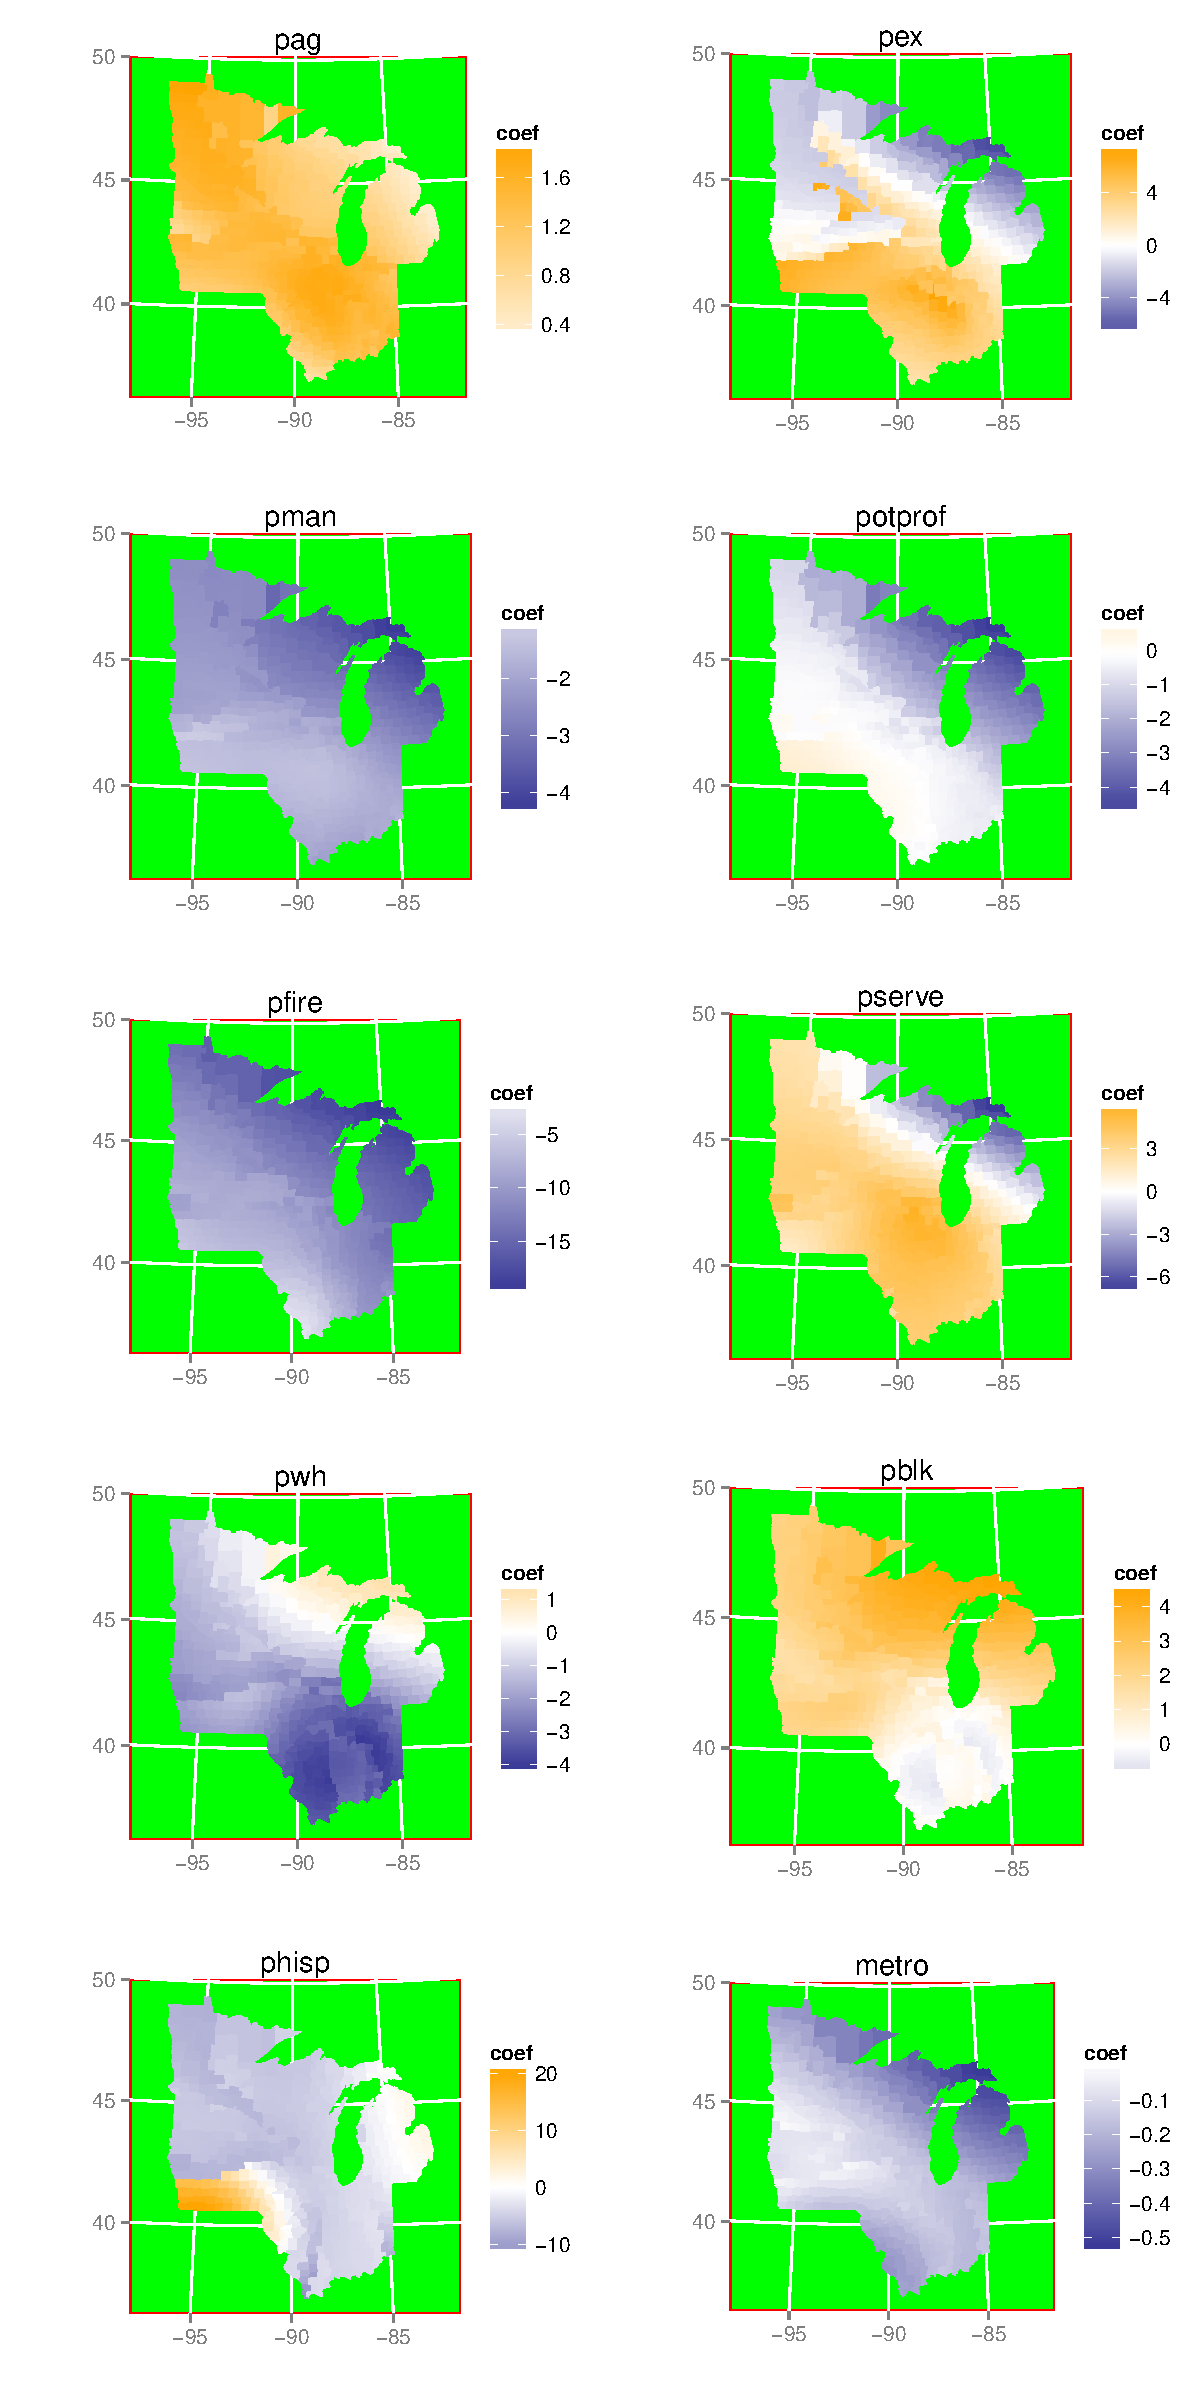
\includegraphics[height=8in]{../../figures/poverty/1970.linear.coefficients.unshrunk.pdf}
			\caption{Coefficient surfaces for the logit of poverty rate, based on the 1970 census and estimated by the unshrunk adaptive elastic net. \label{fig:unshrunk-enet-coefs-1970}}
		\end{center}
	\end{figure}	
	
	\begin{figure}
		\begin{center}
			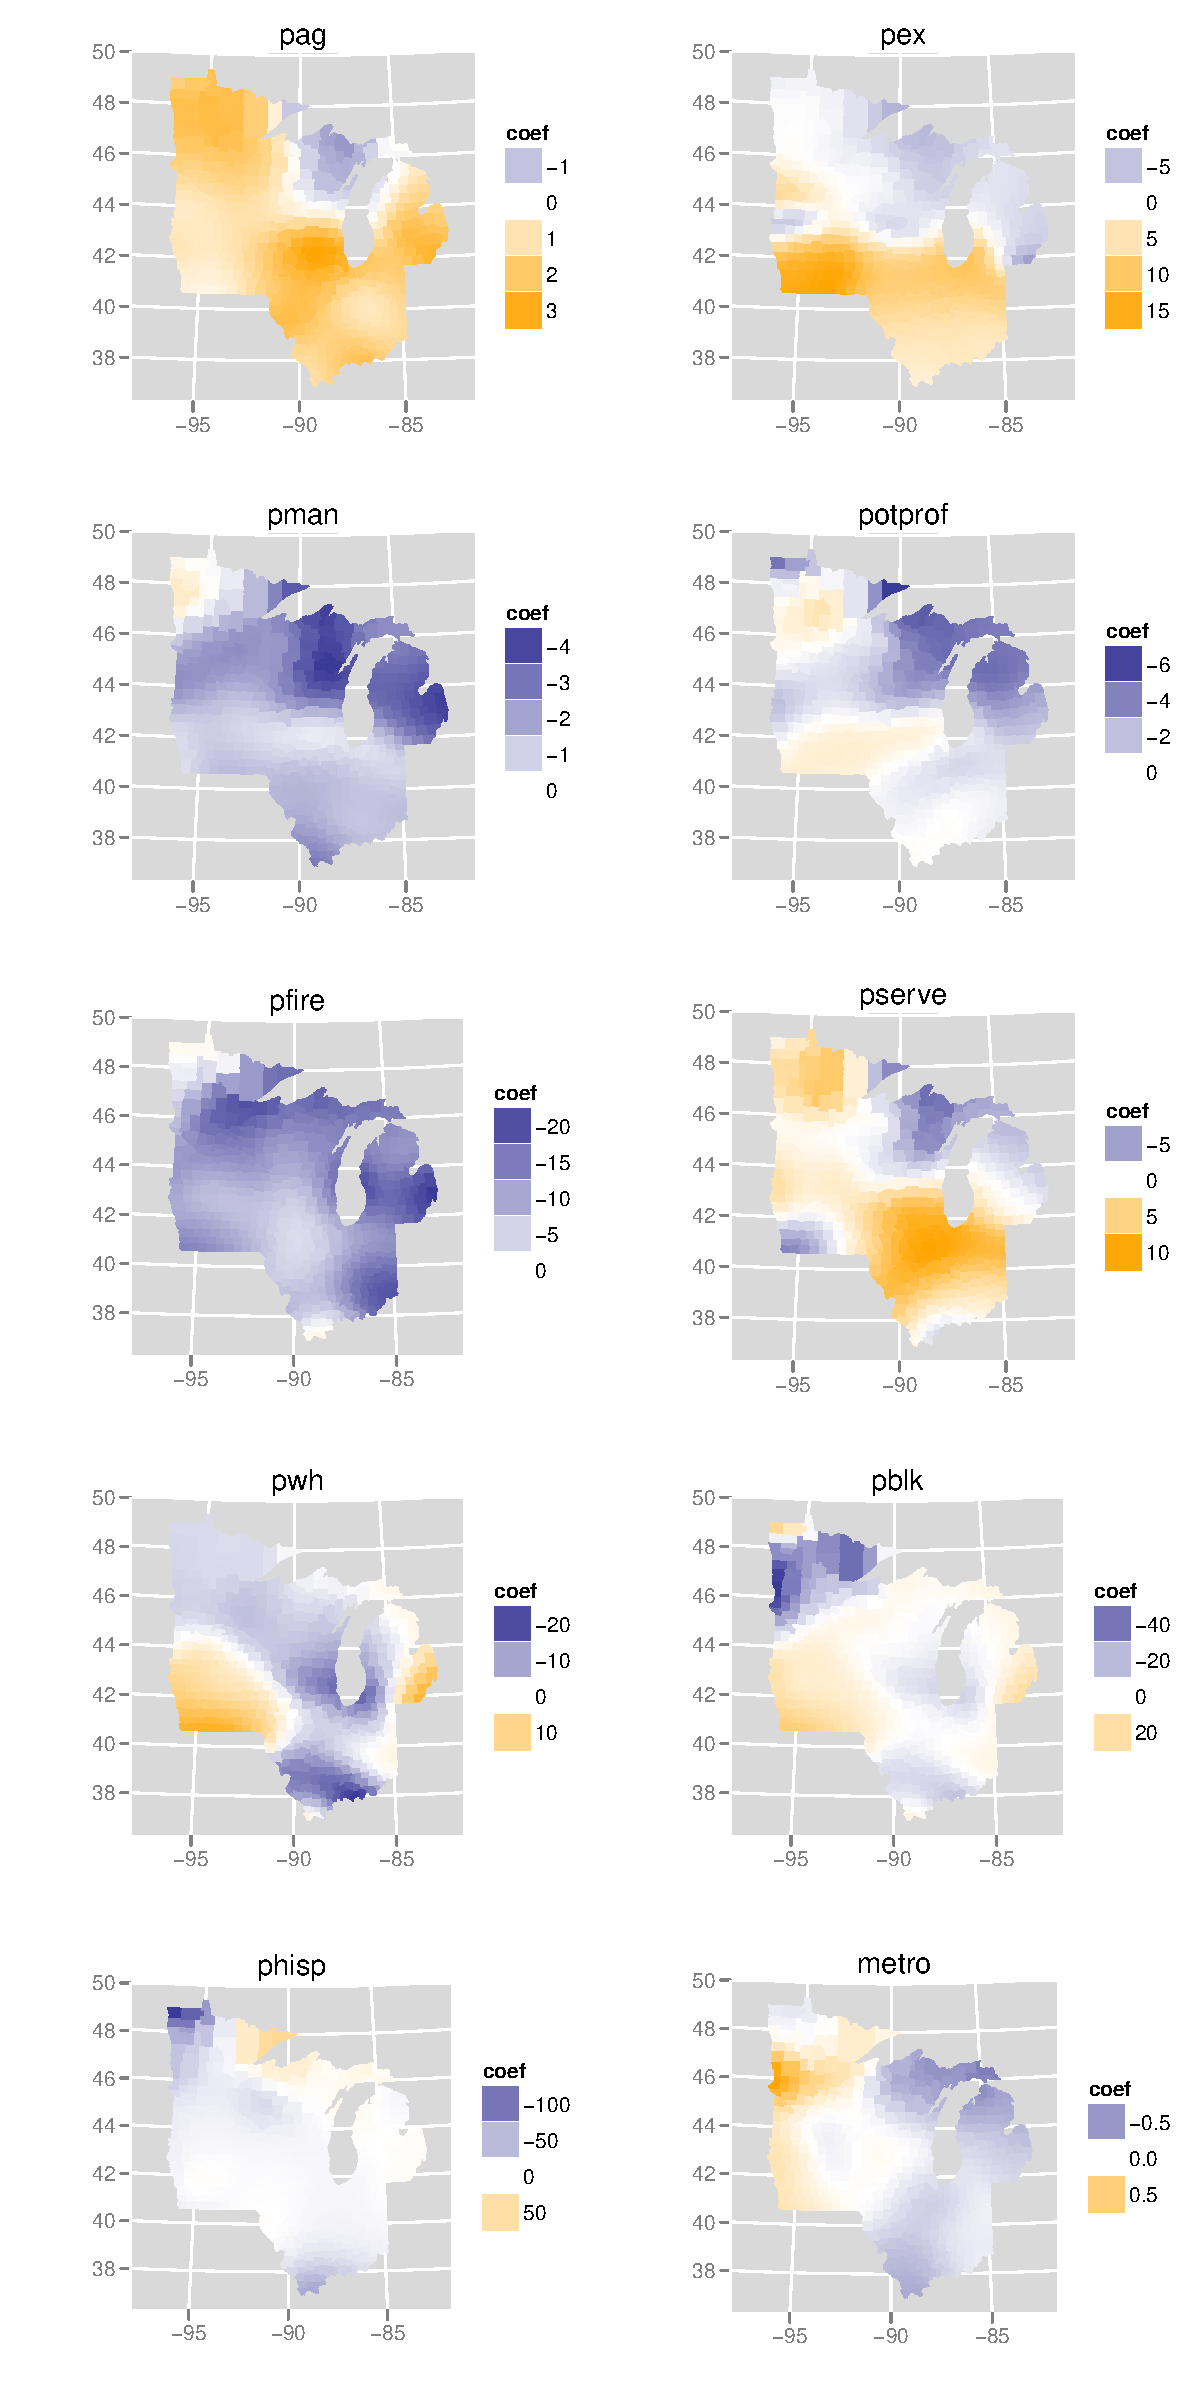
\includegraphics[height=8in]{../../figures/poverty/1970.gwr.pdf}
			\caption{Coefficient surfaces for the logit of poverty rate based on the 1970 census and estimated by base GWR. \label{fig:gwr-coefs-1970}}
		\end{center}
	\end{figure}	
			
	\subsection{Discussion}
	It is immediately apparent that the estimated coefficient surfaces are non-constant for most variables. The same large-scale patterns appear in both figures, but with differences. First of all, the adaptive elastic net has selected a larger bandwidth than base GWR, so there is less variability in the coefficient estimates from the adaptive elastic net. This may be one reason that the adaptive elastic net coefficient estimates are less extreme than those for base GWR. In a model with a logit-transformed proportion as the output, the coefficients can be interpreted as log odds ratios, so, e.g., the estimate of -100 as the coefficient of \verb!phisp! (albeit at the edge of the domain) seems unrealistic.\\
	
	Assessing variable selection for this data is difficult, since the adaptive elastic net almost never removed any variables from the model. Indeed, some coefficients seem nearly constant across the domain. An exception is the coefficient surface for \verb!pex! (mining employment). That surface indicates an interaction whereby the proportion of people working in mining in southern parts of the domain is associated with an increase in the poverty rate, while in northern parts of the domain it is associated with a decrease in the poverty rate.\\

%\end{spacing}

\section{References}
\bibliographystyle{chicago}
\bibliography{../../references/gwr}

\end{document}  